\documentclass[12pt,a4paper]{report}

% --- Packages for styling ---
\usepackage[utf8]{inputenc}
\usepackage[margin=1in]{geometry} % Standard 1-inch margins
\usepackage{graphicx}             % For adding images/logos
\usepackage{setspace}             % For line spacing
\usepackage{xcolor}               % Load color package before titlesec
\usepackage{titlesec}             % For clean heading formatting
\titleformat{\chapter}[block]
  {\normalfont\LARGE\bfseries\color{black}\centering}
  {\chaptername\ \thechapter:\quad}
  {0pt}
  {}
\titleformat{\section}
  {\normalfont\large\bfseries}
  {\thesection\quad}
  {0pt}
  {}
\titleformat{\subsection}
  {\normalfont\large\itshape\raggedright}
  {\thesubsection\quad}
  {0pt}
  {}
\titlespacing*{\chapter}{0pt}{-25pt}{12pt}
\titlespacing*{\section}{0pt}{10pt}{6pt}
\titlespacing*{\subsection}{0pt}{8pt}{4pt}
\usepackage{caption}              % For customizing figure and table captions
\captionsetup[table]{skip=10pt}
\usepackage{array}                %
\usepackage{tikz}                 %This package is for borders
\usetikzlibrary{calc}
\usepackage{eso-pic}              %This is also for borders
\usepackage{tabularx}             % For tables with wrapping columns
\usepackage{array}                % Extended column definitions
\usepackage{ragged2e}             % Better justification controls
\usepackage{tocloft}              % Customize Table of Contents
% Define left-aligned paragraph column type for tables
\newcolumntype{P}[1]{>{\raggedright\arraybackslash}p{#1}}
\usepackage{xurl}                 % For graceful URL line breaks
\usepackage[most]{tcolorbox}      % For highlighted engineering trade-off callouts
\usetikzlibrary{positioning}      %For positioning nodes in diagrams
\usepackage{listings}
\usepackage{xcolor}

% Make tabularx X columns left-aligned (ragged-right)
\renewcommand{\tabularxcolumn}[1]{>{\raggedright\arraybackslash}p{#1}}

% Put a dot after chapter numbers in the Table of Contents
\renewcommand{\cftchapaftersnum}{.}
% ========================================
% Page Border
% ========================================
\AddToShipoutPictureBG{
\begin{tikzpicture}[remember picture,overlay]

\draw[line width=1pt]
($(current page.north west)+(1cm,-1cm)$)
rectangle
($(current page.south east)+(-1cm,1cm)$);

\end{tikzpicture}
}


% Define custom colors for code highlighting
\definecolor{codegreen}{rgb}{0,0.6,0}
\definecolor{codegray}{rgb}{0.5,0.5,0.5}
\definecolor{codepurple}{rgb}{0.58,0,0.82}
\definecolor{backcolour}{rgb}{0.96,0.96,0.94}

% Setup the style
\lstdefinestyle{annexstyle}{
    backgroundcolor=\color{backcolour},   
    commentstyle=\color{codegreen},
    keywordstyle=\color{magenta},
    numberstyle=\tiny\color{codegray},
    stringstyle=\color{codepurple},
    basicstyle=\ttfamily\footnotesize,
    breakatwhitespace=false,         
    breaklines=true,                 
    captionpos=b,                    
    keepspaces=true,                 
    numbers=left,                    
    numbersep=5pt,                  
    showspaces=false,                
    showstringspaces=false,
    showtabs=false,                  
    tabsize=2
}
\lstset{style=annexstyle}

\begin{document}
% Make normal paragraphs fully justified
\justifying

% =========================================================
% PAGE 1: TITLE PAGE (COVER)
% =========================================================
\begin{titlepage}
    \centering
    \vspace*{0.2cm}
    
    % Logo Placeholder (Replace 'example-image' with your logo file name)
    \includegraphics[width=4cm, keepaspectratio]{./images/nrl-logo.png} \\
    \vspace{0.5cm}
    
    {\LARGE \textbf{INTERNSHIP REPORT}} \\
    \vspace{0.8cm}
    
    { A Comprehensive Study of Enterprise Information Security Frameworks and Cybersecurity Practices at Numaligarh Refinery Limited (NRL)} \\
    \vspace{1cm}
    
    {\small Submitted in partial fulfillment of the requirements for the award of the degree of} \\
    \vspace{0.1cm}
    {\large \textbf{BACHELOR OF TECHNOLOGY (B.Tech.) \\ IN \\ COMPUTER SCIENCE AND ENGINEERING}} \\
    \vspace{1.5cm}
    
    \begin{small}
    \textbf{Submitted By} \\
    \vspace{0.2cm}
% =========================================================
% PAGE 1: Table of Names of Students
% =========================================================
   \begin{center}
      
       \begin{tabular}{@{}l l@{}}
            \textbf{Antara Deb} & 232010007007 \\
            \textbf{Avirup Roy} & 232010007010 \\
            \textbf{Darshana Saikia} & 232010007016 \\
            \textbf{Priyangka Das} & 232010007042 \\
            \textbf{Rivleena Khound} & 232010007047 \\
            \textbf{Yashin Syed Hussain} & 242050007014 \\

       \end{tabular}
   \end{center}
   
    
    \vspace{0.5cm}
    \textbf{Under the Guidance of} \\
    \vspace{0.2cm}
    {\large \textbf{Mr. Muhammad Kasim}} \\
    Senior Officer (IIS) \\
    \vspace{0.6cm}
    
    \textbf{Internship Organization} \\
    \vspace{0.2cm}
    Numaligarh Refinery Limited (NRL) \\
    \vspace{0.6cm}
    
    \textbf{Institution} \\
    Barak Valley Engineering College \\
    \vspace{0.6cm}
    
    \textbf{Academic Session} \\
    2024--2027
    \end{small}
\end{titlepage}

% --- Roman numerals for front matter ---
\pagenumbering{roman}

% =========================================================
% PAGE 2: CERTIFICATE
% =========================================================
\newpage

\begin{center}
  \vspace*{1cm}
  {\LARGE \textbf{CERTIFICATE}}
\end{center}
\addcontentsline{toc}{chapter}{CERTIFICATE}
\vspace{1cm}



\begin{center}

This is to certify that the following students,  pursuing the \textbf{Bachelor of Technology (B.Tech.) in Computer Science and Engineering} at \textbf{Barak Valley Engineering College (BVEC)}, has successfully completed their \textbf{internship at Numaligarh Refinery Limited (NRL)} and has submitted the internship report entitled:

\vspace{0.5cm}

\textbf{\emph{"A Comprehensive Study of Enterprise Information Security Frameworks and Cybersecurity Practices at Numaligarh Refinery Limited (NRL)"}}

\vspace{0.5cm}

The report is based on the work carried out by them during the internship period under our guidance and supervision. It reflects their sincere efforts, active participation, and sound understanding of the concepts and practices related to enterprise cybersecurity.

\vspace{0.5cm}

To the best of our knowledge, this report is an original piece of work and has not been submitted, either in whole or in part, to any other university or institution for the award of any degree, diploma, or other academic qualification.

\end{center}
\vspace{2cm}
\begin{center}
      
       \begin{tabular}{@{}l l@{}}
            \textbf{Antara Deb} & 232010007007 \\
            \textbf{Avirup Roy} & 232010007010 \\
            \textbf{Darshana Saikia} & 232010007016 \\
            \textbf{Priyangka Das} & 232010007042 \\
            \textbf{Rivleena Khound} & 232010007047 \\
            \textbf{Yashin Syed Hussain} & 242050007014 \\
       \end{tabular}
   \end{center}
   
\vspace{3cm}

\begin{singlespace}
\noindent

\textbf{Signature of Supervisor} \hfill \textbf{Signature of Head of Department} \\

Name: \_\_\_\_\_\_\_\_\_\_\_\_\_\_\_\_\_\_\_\_\_\_\_\_\_\_\_ \hfill
Name: \_\_\_\_\_\_\_\_\_\_\_\_\_\_\_\_\_\_\_\_\_\_\_\_\_\_\_\_\_\_\_\_\_\_\_\_\_\_\_\_ \\

Designation: \_\_\_\_\_\_\_\_\_\_\_\_\_\_\_\_\_\_\_\_\_\_\_\_\_ \hfill
Department: \_\_\_\_\_\_\_\_\_\_\_\_\_\_\_\_\_\_\_\_\_\_\_\_\_\_\_\_\_\_\_\_\_\_\_\_\\

\end{singlespace}
% =========================================================
% PAGE 3: DECLARATION
% =========================================================
\newpage
\begin{center}
  \vspace*{1cm}
  {\LARGE \textbf{DECLARATION}}
\end{center}
\addcontentsline{toc}{chapter}{DECLARATION}
\vspace{1cm}

We, the undersigned, hereby declare that the internship report entitled \vspace{0.5cm}

\textbf{\emph{"A Comprehensive Study of Enterprise Information Security Frameworks and Cybersecurity Practices at Numaligarh Refinery Limited (NRL)"}}

\vspace{0.5cm}
is a result of the work carried out by us during the course of our internship at \\ \textbf{Numaligarh Refinery Limited (NRL)}. The study has been undertaken as a part of the academic requirements for the award of the degree of \textbf{Bachelor of Technology (B.Tech.) in Computer Science and Engineering} at \textbf{Barak Valley Engineering College (BVEC)}.

We affirm that this report is an original piece of work based on our learning, observations, and practical exposure during the internship. The information and findings presented in this report are true to the best of our knowledge and belief. Wherever references have been made to the work of others, due acknowledgment has been given.

We further declare that this report has not been submitted, either in whole or in part, to any other university or institution for the award of any degree, diploma, or other academic qualification.

\vspace{1cm}
\noindent
\begin{tabularx}{\textwidth}{@{} X r @{}}
    
  % Left side: Student Signatures (stacked vertically with signature lines)
    \begin{minipage}[t]{0.55\textwidth}
        \vspace{0pt}
        \rule{6cm}{0.4pt}\\[4pt]
        Antara Deb -- 232010007007\\[1.0em]
        
        \rule{6cm}{0.4pt}\\[4pt]
        Avirup Roy -- 232010007010\\[1.0em]
        
        \rule{6cm}{0.4pt}\\[4pt]
        Darshana Saikia -- 232010007016\\[1.0em]
        
        \rule{6cm}{0.4pt}\\[4pt]
        Priyangka Das -- 232010007042\\[1.0em]
        
        \rule{6cm}{0.4pt}\\[4pt]
        Rivleena Khound -- 232010007047\\[1.0em]
        
        \rule{6cm}{0.4pt}\\[4pt]
        Yashin Syed Hussain -- 242050007014
    \end{minipage}
    &
    % Right side: Date and Place block
    \begin{minipage}[t][11cm]{0.38\textwidth}
        \vspace{0pt}
        \raggedright
        \vfill
        Date: \rule{4cm}{0.4pt}\\[2em]
        Place: \rule{4cm}{0.4pt}
    \end{minipage}
\end{tabularx}
% XXXXX  DO NOT EDIT THE ABOVE PAGES XXXXX
 
\newpage
\begin{center}
  \vspace*{1cm}
  {\LARGE \textbf{ACKNOWLEDGEMENT}}
\end{center}
\addcontentsline{toc}{chapter}{ACKNOWLEDGEMENT}
\vspace{2cm}
We would like to express our sincere gratitude to \textbf{Numaligarh Refinery Limited (NRL)} for providing us with the valuable opportunity to undertake our internship in the field of cybersecurity and log monitoring. We extend our special thanks to \textbf{Mr. Sangam Panchanan}, Head (T\&D), for granting us this opportunity to learn and for their continuous support throughout the process.
\vspace{1cm}\\
We extend our deepest appreciation to our industry mentor, \textbf{Mr. Muhammad Kasim}, Senior Officer (IIS), NRL, for his invaluable guidance, constant encouragement, and insightful suggestions. His expertise and commitment have been instrumental in shaping the direction and quality of this project. We are indebted to him for his patience, understanding, and the time he has dedicated to reviewing and improving our work.
\vspace{1cm}\\
We would like to express our special gratitude to \textbf{Mr. Himanku Borah}, Senior Consultant, for guiding us through our technical journey. His comprehensive teachings on core cybersecurity topics and the specific technologies utilized at NRL were crucial to our learning experience. He played a pivotal role in helping us conceptualise, decide on, and successfully complete our project, providing unwavering support every step of the way.
\vspace{1cm}\\
We would also like to thank all the officers and staff of the IT and Security departments for their valuable input, which was instrumental in completing the system implementation successfully. Furthermore, we would like to express our sincere appreciation to the faculty members of \textbf{}Barak Valley Engineering College for their academic guidance and continuous motivation during the course of this study.
\vspace{1cm}\\
Lastly, we would like to express our heartfelt gratitude to our families and co-internees for their constant encouragement, love, and understanding. Their unwavering support has been a driving force behind our pursuit of knowledge and personal growth.

\newpage

\newpage
\begin{center}
  \vspace*{1cm}
  {\LARGE \textbf{ABSTRACT}}
\end{center}
\addcontentsline{toc}{chapter}{ABSTRACT}

\vspace{0.5cm}

This report presents a comprehensive study of \textbf{enterprise information security frameworks}, \textbf{digital transformation initiatives}, and \textbf{cybersecurity practices} at Numaligarh Refinery Limited (NRL), culminating in the design and evaluation of a containerized \textbf{Proof-of-Concept (PoC) simulation sandbox}. 

\vspace{0.3cm}
As critical energy infrastructures transition toward \textbf{Industry 4.0}, the convergence of \textbf{Information Technology (IT)} and \textbf{Operational Technology (OT)} introduces complex, high-impact cyber threat surfaces. 

\vspace{0.3cm}
This study first examines NRL's actual digital infrastructure, including:
\begin{itemize}
    \item The implementation of \textbf{India's first 5G Captive Non-Public Network (CNPN)} via BSNL.
    \item A \textbf{3D Digital Twin} utilizing \textbf{Hexagon Asset Lifecycle Information Management (ALIM)}.
    \item A cloud-based \textbf{Integrated Electronic Data and Document Management System (IEDDMS)} hosted on \textbf{Amazon Web Services (AWS)}.
\end{itemize}

\vspace{0.3cm}
To secure this converged environment, NRL leverages an \textbf{AI/ML-driven Managed Detection and Response (MDR)} security posture centered on the \textbf{Airtel Business Secure Intelligent Security Operations Center (iSOC)}, behavior-based \textbf{Next-Generation Endpoint/Extended Detection and Response (EDR/XDR)}, and redundant \textbf{Multi-OEM Next-Generation Firewalls (NGFW)}.

\vspace{0.3cm}
To practically evaluate these enterprise-scale security dynamics, a microservices-based \textbf{PoC simulation sandbox} was developed using \textbf{Docker} and \textbf{Python}:
\begin{itemize}
    \item Custom log collection (\texttt{agent.py}, \texttt{log\_collector.py}) simulating enterprise EDR hosts.
    \item A centralized SIEM analytics engine (\texttt{siem\_server.py}, \texttt{engine.py}) modeling SOC log correlation.
    \item Automated SOAR playbooks (\texttt{block\_ip}, \texttt{isolate\_agent}) demonstrating closed-loop incident containment.
\end{itemize}

\vspace{0.3cm}
This integrated approach bridges the gap between \textbf{theoretical industrial architectures} and \textbf{hands-on defensive engineering}, providing a comprehensive analysis of modern critical national infrastructure protection.
\vspace{0.4cm}
\begin{center}
\renewcommand{\arraystretch}{1.05}
\small
\begin{tabularx}{\textwidth}{|P{3cm}|X|X|P{3.2cm}|}
\hline
\multicolumn{4}{|c|}{\textbf{Core Project Mapping \& Compliance Parameters}} \\ \hline
\textbf{Focus Domain} & \textbf{Enterprise Infrastructure} & \textbf{PoC Sandbox Replicate} & \textbf{Compliance Basis} \\ \hline
Industrial IT/OT & BSNL 5G CNPN \& Hexagon ALIM Twin & \texttt{vulnerable\_app.py} SCADA Honeypot & Purdue Model Zone Segregation \\ \hline
Threat Detection & Airtel Business Secure iSOC (AI/ML) & \texttt{siem\_server.py} \& \texttt{engine.py} Log Ingestion & ISO 27001 ISMS Standards \\ \hline
Incident Response & Redundant NGFW Access Control & \texttt{block\_ip} SOAR Playbook Containment & NIST Cybersecurity Framework \\ \hline
\end{tabularx}
\end{center}
\vspace{0.4cm}

Keywords: Cybersecurity, IT/OT Convergence, 5G CNPN, Managed Detection and Response (MDR), SIEM, SOAR, Proof-of-Concept Sandbox, Critical Infrastructure Protection.

\newpage

\newpage
% =========================================================
% TABLE OF CONTENTS
% =========================================================
\makeatletter
\begin{center}
  {\Large\bfseries Contents}
\end{center}
\vspace{-0.5em}
\@starttoc{toc}
\makeatother

% --- Switch back to regular Arabic numbers for chapters ---
\newpage
\pagenumbering{arabic}

\chapter{INTRODUCTION}

\section{Introduction to SIEM and SOAR}

Modern enterprise Information Technology (IT) and Operational Technology (OT) infrastructures in the industrial sector, particularly within critical petroleum refining environments, generate vast amounts of operational telemetry and security logs. Across systems such as enterprise resource planning (ERP) platforms, cloud-based data repositories, Distributed Control Systems (DCS), Supervisory Control and Data Acquisition (SCADA) networks, and thousands of endpoint devices, daily log generation routinely scales to millions of raw events. Hidden within this massive volume of network and application traffic are critical indicators of compromise (IoCs) that may signal unauthorized access attempts, system anomalies, or Advanced Persistent Threats (APTs) targeting critical national infrastructure.

Security Information and Event Management (SIEM) systems function as the central visibility hub in modern Security Operations Centers (SOCs). A SIEM architecture aggregates heterogeneous log streams from distributed assets, normalizes unstructured log strings into standardized data schemas, applies real-time event correlation rules, and surfaces actionable security incidents. However, in high-throughput industrial environments, security detection alone is insufficient. The latency between identifying a security event and manual mitigation by an analyst presents a critical window of vulnerability.

To address this challenge, Security Orchestration, Automation, and Response (SOAR) frameworks extend the capability of SIEM platforms by automating response playbooks. When a high-severity alert is validated by the SIEM layer, the SOAR module executes automated scripts to isolate compromised endpoints, block malicious traffic at the network perimeter, and alert security personnel at machine speed. 

Within a major national infrastructure asset like Numaligarh Refinery Limited (NRL), security monitoring has transitioned to a proactive, Managed Detection and Response (MDR) security posture. Deployed through the Airtel Business Secure Intelligent SOC (iSOC), this framework integrates AI/ML-driven event analysis and automated containment playbooks to protect both enterprise business applications and industrial control systems.

To study and evaluate these complex enterprise-scale security dynamics in a practical setting, this study develops a containerized Proof-of-Concept (PoC) simulation sandbox alongside the architectural review of NRL's production environment. The PoC sandbox replicates these enterprise controls in a controlled lab environment, establishing a closed-loop defensive pipeline.


\begin{figure}[htbp]
  \centering
  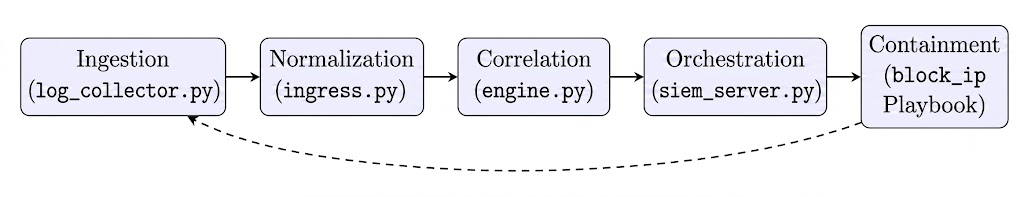
\includegraphics[width=\textwidth, keepaspectratio]{resources/NRL SIEM & SOAR INTERNSHIP REPORT_files/image054.jpg}
  \caption{The closed-loop SIEM and SOAR sandbox execution pipeline.}
  \label{fig:siem-soar-loop}
\end{figure}

The transition from signature-based host defense to behavior-based Next-Gen EDR/XDR is a cornerstone of this posture, as outlined in Table~\ref{tab:av-vs-edr}.

\renewcommand{\arraystretch}{1.3}
\begin{table}[htbp]
\centering
\caption{Security Posture Comparison: Traditional Antivirus vs. Next-Gen EDR/XDR}
\label{tab:av-vs-edr}
\small
\begin{tabularx}{\textwidth}{|p{3cm}|X|X|}
\hline
\textbf{Capability} & \textbf{Traditional Antivirus} & \textbf{Next-Generation EDR/XDR} \\ \hline
\textbf{Detection Basis} & Static signature matching and scheduled file-system scanning. & Behavioral analytics, machine learning, and execution path reconstruction. \\ \hline
\textbf{Threat Focus} & Known malware payloads and executable files. & Fileless attacks, memory injections, zero-day exploits, and lateral movement. \\ \hline
\textbf{Remediation} & Simple file quarantine or deletion (requires signature update). & Autonomous containment, host isolation, Storyline-style process rollback. \\ \hline
\textbf{Connectivity} & Relies on periodic cloud definition database sync. & Real-time telemetry streaming and offline local behavioral agents. \\ \hline
\end{tabularx}
\end{table}

The custom Proof-of-Concept (PoC) sandbox maps these enterprise security operations and controls to localized Python modules as summarized in Table~\ref{tab:concept-mapping}.

\renewcommand{\arraystretch}{1.3}
\begin{table}[htbp]
\centering
\caption{Concept-to-Code Mapping: Enterprise Tooling vs. Custom Simulation Modules}
\label{tab:concept-mapping}
\small
\begin{tabularx}{\textwidth}{|p{3.5cm}|X|X|}
\hline
\textbf{Enterprise Architecture} & \textbf{Primary Operational Role} & \textbf{PoC Sandbox Implementation} \\ \hline
\textbf{EDR/XDR Agents} & Behavioral endpoint monitoring and telemetry aggregation (SentinelOne). & Custom host agent (\texttt{agent.py}) and network logger (\texttt{log\_collector.py}). \\ \hline
\textbf{SIEM \& SOC Core} & AI-driven event normalization, correlation, and alerts (Airtel iSOC). & Central SIEM server (\texttt{siem\_server.py}) and correlation rule engine (\texttt{engine.py}). \\ \hline
\textbf{NGFW \& Perimeter} & Incident containment via dynamic network blocking (Firewalls). & Programmatic SOAR firewall playbook (\texttt{block\_ip} containment script). \\ \hline
\textbf{SCADA \& Target Assets} & Critical OT process controls and plant infrastructure. & SCADA telemetry honeypot service (\texttt{vulnerable\_app.py}). \\ \hline
\end{tabularx}
\end{table}

\newpage
\section{Problem Statement}

Securing an enterprise-scale petroleum refining infrastructure involves addressing three critical operational challenges:

\begin{enumerate}
  \item The IT/OT Convergence and Security Blindspots: The integration of IT systems (such as the cloud-based document management system on AWS) with operational technology (such as the AspenTech plant automation suite) expands the refinery's digital attack surface. Traditional security tools lack visibility across this converged boundary, making it difficult to detect cross-domain threats.
  \item Human Analyst Fatigue and Alert Volumes: The refinery's infrastructure spans more than 1,700 endpoints, servers, and network devices, generating billions of events. Passive monitoring and manual auditing result in delayed response times, leaving a window of opportunity for attackers to move laterally before containment is executed.
  \item High-Availability and Critical National Infrastructure Protection: Refineries are classified as Critical Information Infrastructure (CII). Cyber incidents targeting SCADA systems or plant historians can lead to operational shutdowns, safety hazards, and significant economic impact. This demands a resilient, redundant security architecture with rapid automated incident containment capabilities.
\end{enumerate}

The integration pathway from the field devices up to the cloud-hosted repositories and managed iSOC dashboard is illustrated in Figure~\ref{fig:it-ot-telemetry-flow}.

\begin{figure}[htbp]
\centering
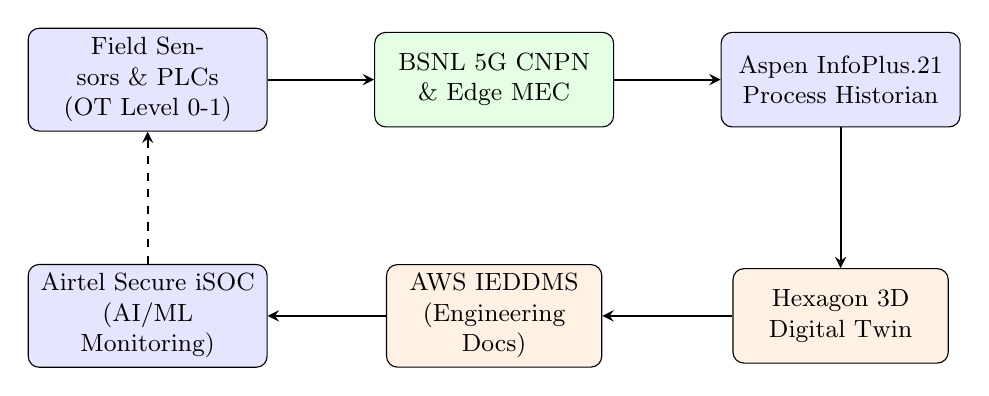
\begin{tikzpicture}[>=stealth, 
  block/.style={rectangle, draw, fill=blue!10, text width=2.8cm, align=center, rounded corners, minimum height=1.2cm, font=\small},
  cloud/.style={rectangle, draw, fill=orange!10, text width=2.5cm, align=center, rounded corners, minimum height=1.2cm, font=\small},
  edge/.style={rectangle, draw, fill=green!10, text width=2.8cm, align=center, rounded corners, minimum height=1.2cm, font=\small}]
  
  \node[block] (sensors) at (0,3) {Field Sensors \& PLCs\\(OT Level 0-1)};
  \node[edge] (mecan) at (4.4,3) {BSNL 5G CNPN\\\& Edge MEC};
  \node[block] (historian) at (8.8,3) {Aspen InfoPlus.21\\Process Historian};
  \node[cloud] (twin) at (8.8,0) {Hexagon 3D\\Digital Twin};
  \node[cloud] (aws) at (4.4,0) {AWS IEDDMS\\(Engineering Docs)};
  \node[block] (soc) at (0,0) {Airtel Secure iSOC\\(AI/ML Monitoring)};
  
  \draw[->, thick] (sensors) -- (mecan);
  \draw[->, thick] (mecan) -- (historian);
  \draw[->, thick] (historian) -- (twin);
  \draw[->, thick] (twin) -- (aws);
  \draw[->, thick] (aws) -- (soc);
  \draw[->, thick, dashed] (soc) -- (sensors);
\end{tikzpicture}
\caption{NRL converged IT/OT telemetry and documentation pathway.}
\label{fig:it-ot-telemetry-flow}
\end{figure}

Securing these flows requires strict alignment with Purdue model levels and security zoning, contrasting traditional IT business architectures with OT industrial configurations as shown in Table~\ref{tab:purdue-model}.

\renewcommand{\arraystretch}{1.3}
\begin{table}[htbp]
\centering
\caption{Purdue Model Levels \& Industrial System Classification}
\label{tab:purdue-model}
\small
\begin{tabularx}{\textwidth}{|P{2.5cm}|P{3cm}|X|X|}
\hline
\textbf{Purdue Level} & \textbf{Domain} & \textbf{Enterprise Systems} & \textbf{Key Security Strategy} \\ \hline
\textbf{Level 4 \& 5} & Enterprise IT & SAP S/4 HANA, ERP, AWS Cloud Hosting, IEDDMS & Central iSOC Monitoring, ZTNA, MFA, Cloud Access IAM \\ \hline
\textbf{Level 3} & Operations DMZ & Historian Data Aggregators, Operations Logs (j5 OMS) & Redundant multi-OEM Firewalls, WAF, API Gateways \\ \hline
\textbf{Level 2} & SCADA/DCS & Supervised Control Consoles, Human Machine Interfaces (HMI) & Redundant network isolation, local historians, session timeouts \\ \hline
\textbf{Level 0 \& 1} & Physical Process & Sensors, Actuators, Programmable Logic Controllers (PLC) & Captive 5G CNPN edge network containment, hardwired interlocks \\ \hline
\end{tabularx}
\end{table}

\section{Significance and Objectives of the Study}

The primary objective of this study is to analyze and evaluate the enterprise information security frameworks, digital transformation initiatives, and cybersecurity operations implemented at Numaligarh Refinery Limited (NRL), and to design a containerized Proof-of-Concept (PoC) simulation sandbox to demonstrate these security controls.

\vspace{0.3cm}
\begin{center}
\small
\begin{tabularx}{\textwidth}{|X|X|X|X|}
\hline
\multicolumn{4}{|c|}{\textbf{Key Performance Statistics \& Expansion Parameters}} \\ \hline
\textbf{9 MMTPA} & \textbf{1,700+} & \textbf{24/7/365} & \textbf{Rs. 28,000 Cr} \\ 
NREP Refining Capacity & Monitored Devices & SOC Monitoring & Projected Investment \\ \hline
\end{tabularx}
\end{center}
\vspace{0.3cm}

The specific objectives of this research are:

\begin{itemize}
  \item To Study the IT/OT Convergence and Industrial Connectivity Architecture: Analyze the integration of BSNL's 5G Captive Non-Public Network (CNPN) and Hexagon ALIM's 3D Digital Twin within the refinery's digital operations.
  \item To Evaluate Cloud-Based Document Management and Security Controls: Investigate the security architecture and document workflows of the cloud-based Integrated Electronic Data and Document Management System (IEDDMS) hosted on AWS.
  \item To Analyze Plant Automation Systems: Examine the deployment of the AspenTech Operational Excellence Suite (including Aspen HYSYS, DMC3, and InfoPlus.21) and its security integration.
  \item To Assess Managed Security Operations: Study the operations, data aggregation flows, and AI/ML-driven correlation capabilities of the Airtel Business iSOC.
  \item To Build and Package a PoC Simulation Sandbox: Implement a containerized microservices stack using Docker and Python to replicate EDR collectors, SIEM servers, and WAF gateways in a simulated lab network.
  \item To Develop and Validate Automated Response Playbooks: Design automated SOAR playbooks (such as client IP blocking and agent isolation) and validate their threat containment velocities against simulated brute-force and web application attacks.
\end{itemize}

\section{Scope and Limitations of the Project}

Scope of the Study

\begin{itemize}
  \item Operational Architecture: Study of the integrated IT and OT networks, including the 5G connectivity backbone, 3D Digital Twin models, operations logs (j5 OMS), and process control systems.
  \item Cloud Infrastructure: Evaluation of AWS cloud security configurations, document access management, and automated approval workflows within the IEDDMS.
  \item Security Center Operations: Investigation of Airtel iSOC monitoring flows, log collection from endpoints and servers, and threat correlation rules.
  \item PoC Sandbox Design: Implementation of custom Python host agents, SIEM correlation engines, and a SCADA web honeypot.
  \item Automated Mitigation Workflows: Empirical testing of closed-loop mitigation playbooks, including IP address blocking and real-time dashboard notifications.
\end{itemize}

Limitations of the Study

\begin{itemize}
  \item Sandbox Scale: While the enterprise analysis covers production-scale systems, the practical threat validation is executed within a controlled, multi-container Docker sandbox rather than directly on NRL's live refinery networks due to plant safety regulations.
  \item Non-Intrusive Analysis: Active security testing, vulnerability scanning, and penetration testing on live refinery production assets were not performed to maintain operational availability and safety.
  \item Data Confidentiality: Specific network topologies, granular firewall access-control lists, active security signatures, and internal incident logs have been abstracted to protect proprietary information.
\end{itemize}

\section{Structure of the Report}

This report is organized into the following chapters:

\begin{itemize}
  \item \textbf{Chapter 1: Introduction} — Outlines the background of enterprise security, defining the problem statement, objectives, scope, and study limitations.
  \item \textbf{Chapter 2: Company Profile} — Details the organizational profile, shareholding patterns, joint ventures, and existing digital and cybersecurity infrastructure of NRL.
  \item \textbf{Chapter 3: Literature Review} — Examines network protocols, core security principles, industry standards (ISO 27001, NIST), and benchmarks commercial and open-source SIEM/SOAR platforms.
  \item \textbf{Chapter 4: Digital Transformation at NRL} — Investigates the deployment of BSNL's 5G Captive Non-Public Network (CNPN) and Hexagon's ALIM for 3D Digital Twin modeling.
  \item \textbf{Chapter 5: Cloud and Plant IT Infrastructure} — Analyzes the cloud-based IEDDMS hosted on AWS and the AspenTech Operational Excellence Suite used for process automation.
  \item \textbf{Chapter 6: Foundational Security Mechanics \& PoC Ingestion} — Deep dive into EDR/XDR, redundant firewalls, and Layer 7 WAF, mapped to the custom Python collectors (\texttt{agent.py}, \texttt{log\_collector.py}) and Ingress APIs (\texttt{ingress.py}).
  \item \textbf{Chapter 7: Cryptographic Security \& Detection Rules} — Cryptographic principles in the enterprise, mapped to the custom SIEM detection rules (\texttt{engine.py}).
  \item \textbf{Chapter 8: Security Operations \& SOAR Playbooks} — Details the operations of the Airtel Secure Intelligent SOC, AI-driven event analysis, and dark web monitoring using Cyble AI, mapped to the automated PoC response playbooks (\texttt{playbooks.py}).
  \item \textbf{Chapter 9: Engineering \& Integration Challenges} — Analyzes the technical challenges associated with IT/OT convergence, system interoperability, and container volume state sync.
  \item \textbf{Chapter 10: Security, Privacy \& Safety Considerations} — Examines data privacy controls (DPDP Act), operational safety, and defensive engineering practices.
  \item \textbf{Chapter 11: System Constraints and Technical Limitations} — Outlines limits in security coverage, remote location connectivity constraints, and skills shortages.
  \item \textbf{Chapter 12: Suggestions, Recommendations \& Future Scope} — Recommends a path forward, including Zero Trust Architectures (ZTA) and advanced machine learning models.
  \item \textbf{Chapter 13: Technical \& Personal Learning Outcomes} — Summarizes key learnings in cloud security, industrial networking, cybersecurity operations, and systems integration.
  \item \textbf{Chapter 14: Conclusion} — Provides a summary of research outcomes, enterprise security postures, and final technical conclusions.
\end{itemize}
\chapter{COMPANY PROFILE}

\section{Overview of Numaligarh Refinery Limited}

Numaligarh Refinery Limited (NRL) is a prestigious Navratna Central Public Sector Enterprise (CPSE) operating under the administrative purview of the Ministry of Petroleum and Natural Gas, Government of India. Earning its elite Navratna designation in December 2025 due to its exceptional operational and financial performance, NRL enjoys substantial strategic autonomy. This corporate elevation provides the organization with greater flexibility in international operations, large-scale financial investments, and independent joint venture decisions without requiring prior government approval, allowing it to compete effectively with global energy conglomerates.

\begin{figure}[htbp]
  \centering
  \includegraphics[width=\textwidth, keepaspectratio]{images/nrl-main-gate.jpg}
  \caption{NRL Main gate}
  \label{fig:nrl-main-gate}
\end{figure}

Located at Numaligarh in the Golaghat district of Assam, NRL operates a highly efficient 3 Million Metric Tonnes Per Annum (MMTPA) crude oil refinery, which is widely recognized as one of the most operationally agile refining setups in the country. The localized refining infrastructure is supported by a 42 TMTPA LPG bottling plant at Numaligarh and primary marketing terminals situated at both Numaligarh and Siliguri. Beyond bulk distribution, NRL has established an extensive downstream retail presence featuring a network of more than 500 retail outlets across the nation. It stands proudly as the single largest petroleum refiner in Northeast India and maintains a dominant global footprint as the country’s largest producer and exporter of high-grade Paraffin Wax.

To secure long-term national energy independence, NRL has embarked on a massive integrated refinery expansion project (NREP) to treble its refining capacity from 3 MMTPA to 9 MMTPA, with an estimated capital investment exceeding Rs. 28,000 Crore. This mega-project fundamentally changes the refinery's logistics, involving the construction of a dedicated Crude Oil Import Terminal at Paradip Port in Odisha and the laying of a 1,640 KM cross-country crude pipeline to transport imported crude oil directly to Numaligarh. Concurrently, NRL is diversifying into petrochemicals by implementing a 360 KTPA Polypropylene project at an estimated cost of Rs. 7,231 Crore. The company consistently demonstrates incredible operational resilience; in FY 2025–26, it processed a record-breaking 3,113 TMT of crude oil, achieving a peak capacity utilization of 103\%—marking the second consecutive year the refinery has operated beyond its rated design capacity.

\section{History and Background}

The historical genesis of NRL is deeply rooted in the historic ``Assam Accord,'' signed on August 15, 1985, between the Government of India, the Government of Assam, and leaders of the Assam Movement to address issues related to regional development, industrialization, and the socio-economic future of the state. Conceived as a major vehicle for rapid industrialization and socio-economic development in the Northeast, the refinery stands as a successful regional corporate execution.

\begin{figure}[htbp]
  \centering
  \includegraphics[width=\textwidth, keepaspectratio]{images/assam-accord.png}
  \caption{The signing of the historic Assam Accord on August 15, 1985}
  \label{fig:assam-accord}
\end{figure}

NRL was formally incorporated as a company on April 22, 1993. The initial 3 MMTPA refining facility was dedicated to the nation by the former Prime Minister of India, Shri Atal Bihari Vajpayee, on July 9, 1999, and commercial operations commenced shortly after in October 2000. Over the past two decades, the refinery has transformed from a localized developmental project into a multi-billion-rupee economic powerhouse for North East India.

\section{Vision, Mission, and Core Values}

NRL operates under a strict strategic framework focused on sustained excellence, digital innovation, and environmental responsibility:
\begin{itemize}
  \item \textbf{Vision}: To be a vibrant, growth-oriented energy company of national standing and global reputation, having core competencies in the refining and marketing of petroleum products, and committed to attaining sustained excellence in performance, safety standards, customer care, and environmental management.
  \item \textbf{Mission}: To develop core competencies in the refining and marketing of petroleum products with a strict focus on international standards regarding safety, quality, and cost optimization.
  \item \textbf{Net-Zero Vision}: Aligning with India’s broader climate goals, NRL has carved out a distinct sustainability roadmap to achieve complete Net-Zero emissions by the year 2038, well ahead of the national 2070 target. In support of this, the company has initiated the setup of a 300 kg/hr (18 MW) Green Hydrogen plant within the refinery premises.
\end{itemize}

\section{Overview of NRL’s IIS and Cybersecurity Infrastructure}

NRL's Information Integration Services (IIS) and digital infrastructure act as the central nervous system across enterprise management, plant automation, and cybersecurity. The company has a rich history of digital evolution: starting as the first oil sector PSU to implement Ramco ERP in 1998, migrating to SAP R/3 in 2005, upgrading to SAP ECC 6.0 in 2011, and ultimately migrating to modern SAP S/4 HANA integrated with IBM Business Automation Workflow (BAW) in 2022 to digitize all key business processes. Plant operations are driven by the AspenTech Operational Excellence Suite (including Aspen HYSYS, DMC3, and InfoPlus.21) alongside the SampleManager LIMS for certified quality control workflows.

From a cybersecurity perspective, NRL has maintained a rigorous ISO 27001 Information Security Management System (ISMS) certification since June 2009. The refinery’s digital infrastructure is safeguarded by an enterprise-grade Managed Detection and Response (MDR) Security Operations Center (SOC) framework leveraging AI-driven log correlation, 24/7 endpoint/network defense, and automated threat hunting. NRL's double-layered protection architecture features Next-Generation Firewalls (NGFWs) deployed from two completely different OEMs within the OT network to maximize defensive redundancy. Recent key security initiatives include:

\begin{figure}[htbp]
  \centering
  \includegraphics[width=\textwidth, keepaspectratio]{images/best-ciso-award.jpg}
  \caption{Best CISO of the Year award at the 2nd Bharat PSU Manthan 2026}
  \label{fig:best-ciso-award}
\end{figure}

NRL's digital excellence has earned it extensive national acclaim, including the Excellence in Cyber Security and SOC Implementation honour at the 3rd PSU Transformation Awards, the Best use of Automation \& Digital Technologies at the Governance Now 11th PSU Awards, and the Best CISO of The Year award at the 2nd Bharat PSU Manthan 2026.

\section{Shareholding Patterns}

As of the current operational cycle, NRL possesses an Authorized Share Capital of Rs. 5,000 Crore and a Paid-up Share Capital of Rs. 1,758.99 Crore. The company features a highly structured public sector equity distribution:

\renewcommand{\arraystretch}{1.3}
\begin{table}[htbp]
\centering
\caption{NRL Equity Shareholding Pattern}
\label{tab:shareholding}
\footnotesize
\begin{tabularx}{\textwidth}{|X|X|X|X|}
\hline
Name of shareholder & Number of shares & \% of shareholding & Paid-up value of Rs. 10 each \\ \hline
Oil India Limited & 1,22,47,85,313 & 69.63 & Rs.12,24,78,53,130 \\ \hline
Govt. of Assam & 45,73,37,481 & 26.00 & Rs.4,57,33,74,810 \\ \hline
Engineers India Limited & 7,68,67,541 & 4.37 & Rs.76,86,75,410 \\ \hline
Nominee of OIL & 12 & - & Rs. 120 \\ \hline
Nominee of Govt. of Assam & 14 & - & Rs. 140 \\ \hline
Total & 1,75,89,90,361 & 100.00 & Rs.17,58,99,03,610 \\ \hline
\end{tabularx}
\end{table}

\begin{figure}[htbp]
  \centering
  \includegraphics[width=\textwidth, keepaspectratio]{images/shareholding-pattern.png}
  \caption{Shareholding Pattern}
  \label{fig:shareholding-pattern}
\end{figure}

\section{Alliances and Joint Ventures}

To support its tripling capacity expansion and cross-border commercial strategy, NRL has entered into major alliances and joint ventures:
\begin{itemize}
  \item \textbf{Upstream \& Downstream Integration}: Direct B2B operational integration via unified SAP pipelines with major industry players, including IOCL, BPCL, HPCL, ONGC, and Nayara Energy.
  \item \textbf{Assam Bio-Refinery Pvt. Ltd.}: A pioneering joint venture focused on setting up a bamboo-based 2G bio-refinery, diversifying NRL's portfolio into renewable biofuels.
  \item \textbf{Northeast Gas Grid Project}: Strategic alignment and equity participation in building the regional natural gas transmission grid.
  \item \textbf{International Alliances}: The construction and operation of the historic Indo-Bangla Friendship Pipeline, spanning from Siliguri to Bangladesh, allowing NRL to smoothly export middle distillates internationally.
  \item \textbf{Logistics \& Supply Expansion}: Massive supply-chain infrastructure joint ventures, including a dedicated Crude Oil Import Terminal at Paradip Port (Odisha) connected to the refinery via a newly laid 1,640 KM cross-country crude pipeline.
\end{itemize}

\newpage
\chapter{LITERATURE REVIEW}

This chapter establishes the theoretical and enterprise context within which this SIEM and SOAR platform operates. Before engineering a modern Security Information and Event Management (SIEM) and Security Orchestration, Automation, and Response (SOAR) architecture, it is critical to evaluate the conceptual evolution of log analytics, review global cybersecurity compliance frameworks, and benchmark existing enterprise solutions. This review serves to define the technical requirements of the simulated enterprise security architecture and illuminates the current research and operational gaps that this software-centric deployment addresses.

\section{Sources of Literature}

The foundational literature compiled for this research spans three distinct domains:
\begin{enumerate}
  \item \textbf{Vendor Specifications and Technical Blueprints}: In-depth technical documentation of leading commercial and open-source log aggregation systems (such as Splunk, Elastic Security, Logstash, Filebeat, and Wazuh), focusing on data ingestion models, log parsing pipelines, and distributed agent configurations.
  \item \textbf{Global Cybersecurity Frameworks}: Official documentation published by the National Institute of Standards and Technology (NIST Cybersecurity Framework), the International Organization for Standardization (ISO/IEC 27001 ISMS standard), the Purdue Model for Industrial Control Systems, and the MITRE Corporation (ATT\&CK Matrix for enterprise threat mapping).
  \item \textbf{Market Analysis and Sector Intelligence}: Contemporary cybersecurity industry whitepapers charting major technology consolidations and architectural shifts within modern enterprise Security Operations Centres (SOCs).
\end{enumerate}

\section{Conceptual Security Background}

\subsection{The Purdue Model for IT/OT Segmentation}

In industrial security architectures, enterprise networks must be strictly isolated from plant floor control systems. The industry standard for mapping these zones is the \textbf{Purdue Model}, which structures systems into distinct logical levels of trust. This segregation prevents threat propagation; an adversary compromising a corporate email account in the IT zone cannot directly access SCADA systems or PLCs in the OT zone.

\renewcommand{\arraystretch}{1.3}
\begin{table}[htbp]
\centering
\caption{Purdue Model Levels \& System Classification}
\label{tab:purdue-model}
\footnotesize
\begin{tabularx}{\textwidth}{|p{1.8cm}|p{2.5cm}|X|X|}
\hline
Level & Zone & Description & Representative Systems (NRL Context) \\ \hline
Level 4 / 5 & Enterprise IT & Standard business operations and ERP applications. & SAP S/4 HANA, AWS engineering document cloud (IEDDMS), corporate offices. \\ \hline
Level 3.5 & Industrial DMZ & Security boundary mediating data exchange between IT and OT. & Redundant Next-Generation Firewalls (NGFW), FortiAnalyzer log collectors. \\ \hline
Level 3 & Site Operations & Systems aggregating operational data and monitoring units. & Aspen InfoPlus.21 (IP21) historian, Hexagon j5 OMS servers. \\ \hline
Level 2 & Supervisory Control & Operator consoles, HMIs, and plant-wide control software. & Distributed Control Systems (DCS), supervisory SCADA stations. \\ \hline
Level 1 & Local Control & Direct control of physical processes. & PLCs, Remote Terminal Units (RTUs), local controller loops. \\ \hline
Level 0 & Physical Process & The physical refining equipment. & Field sensors, control valves, pumps, heaters, and boilers. \\ \hline
\end{tabularx}
\end{table}

\subsection{Managed Detection and Response (MDR) in Critical Infrastructure}

Refineries are classified as Critical Information Infrastructure (CII), where system downtime or security incidents impact national security. Traditional localized Security Operations Centers (SOCs) struggle to maintain 24/7/365 coverage due to geographical constraints and the talent shortage in cybersecurity. Evolving threat landscapes demand \textbf{Managed Detection and Response (MDR)}, where a dedicated external partner (e.g. Airtel Business Secure iSOC) monitors telemetry round-the-clock, enriches events with global threat intelligence, and triggers automated playbooks to contain threats before lateral movement occurs.

\subsection{Next-Gen EDR/XDR vs. Legacy Antivirus}

Traditional antivirus solutions depend heavily on static signature databases and scheduled system scans. Consequently, they fail against modern threat vectors such as fileless malware, memory injection attacks, and fast-moving ransomware. Next-Generation \textbf{Endpoint Detection and Response (EDR/XDR)} systems run lightweight agent engines locally on hosts. These engines use behavior analytics and machine learning to reconstruct execution processes (e.g. SentinelOne Storyline), detecting and isolating anomalous behavior at machine speed even when offline.

\renewcommand{\arraystretch}{1.3}
\begin{table}[htbp]
\centering
\caption{Traditional vs. Next-Gen Security Controls}
\label{tab:traditional-vs-nextgen}
\footnotesize
\begin{tabularx}{\textwidth}{|p{2.8cm}|X|X|}
\hline
Operational Capability & Traditional / Legacy Approach & Modern Next-Generation Controls \\ \hline
\textbf{Endpoint Defense} & Static signature matches, file-based scanning, manual virus database updates. & Behavior analytics, machine learning execution tracking, fileless malware detection, autonomous agent network isolation (SentinelOne). \\ \hline
\textbf{Network Boundaries} & Single perimeter firewall separating corporate IT from the internet. & Redundant, double-layered Next-Generation Firewalls (NGFW) from different OEMs at IT/OT boundaries. \\ \hline
\textbf{Threat Operations} & Standalone SIEM log search, manual incident response, alert fatigue. & Managed Detection and Response (MDR), AI/ML-assisted log correlation, automated SOAR playbooks (Airtel Business iSOC). \\ \hline
\textbf{Threat Intelligence} & Reactive updates on known indicators of compromise (IoC) from vendor bulletins. & Proactive external threat intelligence and dark web credential scanning (Cyble AI). \\ \hline
\end{tabularx}
\end{table}

\section{Review of Existing SIEM/SOAR Platforms}

The corporate security landscape has experienced major structural changes driven by enterprise technology consolidation. Cisco finalized its acquisition of Splunk, shifting Splunk's trajectory deeper into consolidated cloud ecosystems. Concurrently, IBM divested its QRadar SaaS components to Palo Alto Networks, with legacy on-premise components transitioning to end-of-life status. These market realignments have driven increased interest toward modular open-source log pipelines (e.g., Filebeat and Logstash) and customizable platforms (e.g., Wazuh).

\renewcommand{\arraystretch}{1.3}
\begin{table}[htbp]
\centering
\caption{SIEM and SOAR Platform Benchmarking}
\label{tab:platform-comparison}
\renewcommand{\arraystretch}{1.3}
\footnotesize
\begin{tabularx}{\textwidth}{|>{\raggedright\arraybackslash}p{2.2cm}|>{\raggedright\arraybackslash}X|>{\raggedright\arraybackslash}X|>{\raggedright\arraybackslash}X|>{\raggedright\arraybackslash}X|}\hline
Platform Name & Deployment Type & System Architecture & Advanced Detection \& SOAR Approach & Primary Architectural Trade-off \\ \hline
Splunk Enterprise Security & Commercial Enterprise & Centralised heavy ingestion \& index search cluster & Stateful rule mapping + UEBA; Integrated Splunk SOAR / Phantom playbooks & High licensing costs scaling linearly with daily log volume. \\ \hline
Elastic Security & Commercial (Open Core) & Elasticsearch data nodes + Logstash/Filebeat pipeline + Kibana UI & EQL-based correlation rules + Machine Learning; Webhook-driven alerts & High ingest speed; complex cluster setup and resource footprint. \\ \hline
Wazuh & Open Source & Distributed architecture: Indexer, Manager, \& Active Host Agents & Signature checking + Active Response scripts & Zero licensing overhead; demands substantial in-house setup and tuning. \\ \hline
This Project Sandbox & Purpose-Built Microservices Prototype & Containerized: Ingress Gateway + Logstash/Filebeat + Python Engines (\texttt{engine.py}, \texttt{playbooks.py}) & Stateful multi-source correlation rules + Automated Python response playbooks (\texttt{playbooks.py}) & Lightweight, fully transparent codebase; scoped for lab/sandbox evaluation scale. \\ \hline
\end{tabularx}
\end{table}

\section{Research \& Engineering Gap}

While enterprise commercial systems possess comprehensive feature sets, they operate as proprietary, resource-heavy ``black-box'' appliances that hide underlying data processing flows from engineers. Conversely, standard academic or entry-level monitoring projects frequently suffer from scope under-fitting, typically parsing isolated text log files using basic regular expressions on a single machine without automated response capabilities.

Consequently, a distinct engineering gap exists between functionally opaque production systems and basic scripts that fail to demonstrate real-time ingestion pipelines, multi-source event correlation, or closed-loop response workflows. This project addresses this gap by engineering a transparent, first-principles platform that exposes the entire operational pipeline: from multi-agent log forwarding and Flask API ingress to real-time threat detection, automated SOAR containment, attack target simulation, and SOC dashboard rendering.

\section{Statement of the Problem}

Enterprise security operations struggle with severe inefficiencies stemming from massive log volumes, fragmented data sources, and slow manual incident triage. When critical indicators of compromise are scattered across web servers, databases, and application endpoints, standalone log viewers fail to connect related events. Furthermore, purely manual incident response workflows cannot react quickly enough to contain active attacks before system degradation occurs.

This project directly addresses this operational challenge by designing, implementing, and validating a containerised, multi-component microservice architecture. The system continuously ingests telemetry streams, normalises incoming logs into structured data models, evaluates stateful correlation rules, executes automated remediation playbooks, and renders active threats on a the industry concepts, compliance standards, and architectural paradigms evaluated in this chapter establish the theoretical foundation for the platform. By combining centralised log shipping with real-time correlation and automated response orchestration, the platform provides a robust framework for the methodology and detailed system architecture detailed in subsequent chapters.

\newpage
\chapter{DIGITAL TRANSFORMATION \& INDUSTRIAL CONNECTIVITY}

This chapter details Numaligarh Refinery Limited's (NRL) strategic digital transformation initiatives and modern industrial IT/OT architectures. To support the NREP 9 MMTPA capacity expansion, NRL has deployed advanced networking, digital asset modeling, cloud storage, and process optimization solutions. These initiatives establish a highly secure, reliable, and integrated digital ecosystem across the enterprise.

\section{BSNL 5G Captive Non-Public Network (CNPN)}

In August 2025, NRL deployed India's first 5G Captive Non-Public Network (CNPN) in the refining sector, in partnership with Bharat Sanchar Nigam Limited (BSNL). The private 5G network provides the ultra-reliable, low-latency communication (URLLC) and high bandwidth needed to connect critical refinery operations:
\begin{itemize}
  \item \textbf{High-Speed Ingestion}: Real-time aggregation of process telemetry from thousands of field sensors and IoT transmitters across the refinery floor.
  \item \textbf{Immersive Workforce Training}: Seamless integration of Augmented, Virtual, and Mixed Reality (AR/VR/MR) systems for workforce training and remote maintenance assistance.
  \item \textbf{Edge Computing (MEC)}: Combining private 5G spectrum with Multi-access Edge Computing (MEC) keeps critical control-plane data processing localized at the plant edge, reducing central cloud backhaul and improving operational resilience.
\end{itemize}

\section{3D Digital Twin \& Operations Management}

NRL has digitized physical plant assets and operational logs to create a unified operational picture:
\begin{itemize}
  \item \textbf{Hexagon ALIM (Asset Lifecycle Information Management)}: Maintains a spatially accurate 3D Digital Twin and data-centric master model of the refinery's physical infrastructure. ALIM links engineering design blueprints directly to real-time operations, ensuring data consistency throughout the asset lifecycle.
  \item \textbf{Hexagon j5 OMS (Operations Management Solution)}: Digitizes shift handover sheets, operator round logs, and standing orders. It replaces manual paper-based logs, minimizing human error during shift transitions.
  \item \textbf{Historian Integration}: Utilizes the j5 Connector for AspenTech to pull process historian tags directly into shift logs, providing operators with context-aware process telemetry during shift handovers.
\end{itemize}

\section{AWS-Based Document Management (IEDDMS)}

To manage the massive volume of technical drawings and blueprints for the 9 MMTPA Refinery Expansion Project (NREP), NRL migrated its Integrated Electronic Data and Document Management System (IEDDMS) to Amazon Web Services (AWS), implemented in collaboration with AWS partner Minfy Technologies:
\begin{itemize}
  \item \textbf{Serverless Processing Pipeline}: Files uploaded to Amazon S3 trigger AWS Lambda and Step Functions. These serverless workflows use AWS Textract to perform Optical Character Recognition (OCR), metadata extraction, and automated indexing.
  \item \textbf{Secure Cloud Hosting}: Deployed inside a secured Virtual Private Cloud (VPC) with strict IAM (Identity and Access Management) controls and data encryption at rest (AES-256) and in transit (TLS 1.3).
  \item \textbf{Global Collaboration}: Enables secure, high-availability document access for international vendors and contractors, accelerating engineering approval workflows.
\end{itemize}

\section{AspenTech Operational Excellence Suite}

Operational optimization and process historians reside in the OT control layers, driving refinery safety and throughput:
\begin{itemize}
  \item \textbf{Aspen HYSYS}: Used for process engineering simulation and thermodynamic calculations. It creates digital twins of physical refinery units to predict heat exchanger fouling, optimizing maintenance schedules.
  \item \textbf{Aspen DMC3 (Dynamic Matrix Control)}: Deployed for Advanced Process Control (APC) inside major refinery units (CDU/VDU). DMC3 utilizes multivariable predictive control to maximize CDU/VDU throughput and product yield.
  \item \textbf{Aspen InfoPlus.21 (IP21)}: Serves as the primary manufacturing data historian. It aggregates millisecond-level time-series data from Distributed Control Systems (DCS) and SCADA networks, providing a centralized data repository for plant-wide analytics.
\end{itemize}

\section{Industrial Data Integration Architecture}

The edge capture, transport, control, and document management systems operate as a tightly integrated workflow. Telemetry streams from field instruments over the private 5G CNPN to MEC nodes and edge gateways, which forward records to the DCS control loops and the Aspen IP21 historian. The Hexagon 3D Digital Twin subscribes to IP21 historian tags, updating 3D models with flow, pressure, and temperature values. Concurrently, the cloud-hosted IEDDMS provides engineering document support, integrating drawings with asset management systems.

To illustrate the technical connectivity, the table below documents the primary integration points across the converged IT/OT ecosystem:

\renewcommand{\arraystretch}{1.3}
\begin{table}[htbp]
\centering
\caption{NRL Industrial IT/OT Primary Integration Points}
\label{tab:integration-points}
\footnotesize
\begin{tabularx}{\textwidth}{|p{3cm}|p{3.5cm}|X|}
\hline
Source Interface & Destination Interface & Operational Telemetry \& Data Exchanged \\ \hline
5G CNPN & MEC / Edge Compute & Aggregates IoT sensor telemetry and handles protocol translation. \\ \hline
Edge Gateways & DCS / SCADA & Routes time-series data using OPC/Modbus to Aspen InfoPlus.21. \\ \hline
InfoPlus.21 (IP21) & Hexagon Digital Twin & Streams real-time flow, pressure, and temperature tags to update the 3D site model. \\ \hline
AWS IEDDMS (S3) & Hexagon / Asset Systems & Links engineering drawings, approval workflows, and manuals to 3D asset nodes. \\ \hline
Cross-Domain APIs & SIEM Collectors & Forwards security events and API logs via REST/HTTPS to cybersecurity monitoring systems. \\ \hline
\end{tabularx}
\end{table}

The integration points described above establish the industrial data fabric analysed in Chapter 5.

\newpage
\chapter{SYSTEM ARCHITECTURE}

\begin{figure}[htbp]
  \centering
  \includegraphics[width=\linewidth, height=0.6\textheight, keepaspectratio]{images/system-architecture-flow.png}
  \caption{System Architecture Flow}
  \label{fig:system-architecture-flow}
\end{figure}

This Security Information and Event Management (SIEM) and Security Orchestration, Automation, and Response (SOAR) platform is engineered as a decoupled, microservices-driven architecture. Each containerised module is assigned a specific function within the continuous telemetry processing, stream normalisation, threat correlation, and automated incident response lifecycle. To ensure absolute platform portability, reproducibility, and environment isolation, all components are packaged and orchestrated via Docker and Docker Compose.

In the industry context of Numaligarh Refinery Limited (NRL), system architecture spans five distinct Purdue levels: Level 0/1 (field instruments and PLCs), Level 2 (DCS supervisory control and HMIs), Level 3 (process historians and j5 operations logs), Level 3.5 (Operations DMZ), and Level 4/5 (Enterprise IT networks, SAP S/4 HANA, and AWS cloud storage).

The sandbox project replicates these exact structural controls. As illustrated in the architectural overview, system telemetry flows through a deterministic, unidirectional pipeline before executing an automated defence action. Security logs generated by the target web application (\texttt{vulnerable\_app.py}) and log shipping agents (\texttt{agent.py}, \texttt{log\_collector.py}) are securely routed to the central Ingress API (\texttt{ingress.py}), where raw records are normalised into structured data attributes. The events are then evaluated by the SIEM detection engine (\texttt{engine.py}) against stateful correlation rules. Upon identifying an indicator of compromise, structured alert objects (SIEM Alert Object Models) are instantiated, instantly triggering the SOAR orchestration module (\texttt{playbooks.py}) to execute automated remediation workflows (e.g., dynamic IP blocking). The management dashboard operates asynchronously as a decoupled read-only interface, querying active system metrics and alert states without impacting the core ingestion throughput.

\section{Microservice Component Descriptions}

\subsection{Distributed Log Shipping and Agent Boundary}

The ingestion boundary comprises decoupled log collection agents and shipping daemons deployed across target environments.
\begin{itemize}
  \item \textbf{Theoretical Context (NRL)}: Endpoint telemetry is harvested from more than 1,700 endpoints, servers, and central databases. In addition, OT-domain gateways stream industrial event logs, process alarms, and operator shift records generated inside the \textbf{Hexagon j5 Operations Management Solution (OMS)}. These logs capture operational handovers and process historian exceptions.
  \item \textbf{Sandbox Simulation}: Lightweight Python scripts (\texttt{agent.py} and \texttt{log\_collector.py}) act as endpoint EDR and network log collectors. They poll local system logs, encapsulate raw event text into standardized JSON payloads, attach host identifiers, and stream them via secure HTTP POST requests to the central Ingress API.
  \item \textbf{Filebeat \& Logstash Ingestion}: Filebeat intercepts event logs and ships them to Logstash, which runs pattern matching (Grok filters) to parse unstructured strings into normalized fields (extracting variables such as client IP addresses, HTTP response codes, and timestamps).
\end{itemize}

\subsection{Central Ingress API Gateway}

The primary entry point for distributed telemetry is the Ingress API gateway (\texttt{ingress.py}), simulating Layer 7 web security protection.
\begin{itemize}
  \item \textbf{Theoretical Context (NRL)}: The refinery protects its public interfaces and B2B vendor APIs using a Web Application Firewall (WAF) to perform deep packet inspection at Layer 7. The WAF blocks OWASP Top 10 vulnerabilities (SQLi, XSS, directory traversal) and protects the cloud-hosted \textbf{Integrated Electronic Data and Document Management System (IEDDMS)} running on AWS. Deployed in collaboration with Minfy Technologies, this system manages all blueprints and engineering drawings for the \textbf{9 MMTPA Refinery Expansion Project (NREP)}.
  \item \textbf{Sandbox Simulation}: The custom Python Ingress API gateway performs payload validation, strips malicious parameters, extracts client socket IPs, and pushes sanitised records to the SIEM processing queues.
\end{itemize}

\subsection{SIEM Detection and Correlation Core}

The analytical processing layer is driven by the core SIEM detection engine (\texttt{engine.py}).
\begin{itemize}
  \item \textbf{Theoretical Context (NRL)}: Managed security operations are centered in the \textbf{Airtel Business Secure Intelligent SOC (iSOC)}. The iSOC implements automated AI/ML models to analyze, parse, and correlate event telemetry from different network zones (IT business vs. OT SCADA), filtering out noise and false positives to identify real indicator-of-compromise (IoC) threats.
  \item \textbf{Sandbox Simulation}: The custom correlation engine implements stateful algorithms over sliding chronological windows to detect error rate spikes, brute-force access attempts, and scanning anomalies, generating structured alert objects.
\end{itemize}

\subsection{SOAR Orchestration and Playbook Engine}

The SOAR engine (\texttt{playbooks.py}) provides automated, closed-loop incident containment.
\begin{itemize}
  \item \textbf{Theoretical Context (NRL)}: When a high-severity alert is validated, automated SOAR workflows run across the network infrastructure. They execute endpoint containment (via SentinelOne EDR/XDR) and inject perimeter IP blocks across redundant Next-Generation Firewalls (NGFW) to prevent lateral movement.
  \item \textbf{Sandbox Simulation}: The SOAR engine processes the SIEM alert objects, determines severity, and executes the appropriate Python playbook, such as dynamically appending the adversary IP to the active database blocklist.
\end{itemize}

\subsection{Vulnerable Target Application}

To validate the detection and response pipeline, the platform incorporates a dedicated target web application (\texttt{vulnerable\_app.py}).
\begin{itemize}
  \item \textbf{Theoretical Context (NRL)}: This represents the plant operational control layers. The refinery utilizes the \textbf{AspenTech Operational Excellence Suite}, including \textbf{Aspen HYSYS} for process simulation (such as predicting heat exchanger fouling) and \textbf{Aspen DMC3} for Advanced Process Control (APC) inside major refinery units (e.g., Crude and Vacuum Distillation Units - CDU/VDU). Process control is managed via Distributed Control Systems (DCS) and SCADA.
  \item \textbf{Sandbox Simulation}: The custom target app simulates a SCADA HMI dashboard, exposing heater temperatures, pressures, and flow rates while displaying vulnerabilities to allow brute-force, injection, and scanning attack scenarios.
\end{itemize}

\subsection{SOC Monitoring Dashboard}

The user-facing presentation fabric is delivered via a web interface managed by dashboard routing logic.
\begin{itemize}
  \item \textbf{Theoretical Context (NRL)}: Security teams monitor the refinery's enterprise posture using unified console screens that aggregate threat reports, active firewall blocklists, and external intelligence updates from \textbf{Cyble AI} (monitoring dark web sources for leaked credentials).
  \item \textbf{Sandbox Simulation}: The web-based SOC dashboard runs asynchronously, rendering active events, alert metrics, blocked IPs, and playbook execution histories.
\end{itemize}

\section{Asynchronous Telemetry Data Flow}

The execution path of a security event through this platform follows an explicit chronological progression:
\begin{enumerate}
  \item Telemetry Generation: An external actor interacts with the SCADA honeypot, or process sensors generate logs.
  \item Secure Transmission: Log shipping agents or Filebeat/Logstash intercept the event and forward it to the Ingress API.
  \item Normalisation and Ingestion: The Ingress module normalises raw text, stamps it with host attributes, and validates schemas.
  \item Correlation Analysis: The engine scans incoming records against active rule signatures inside sliding windows.
  \item Alert Escalation: A structured security alert object is instantiated upon rule violation.
  \item Playbook Execution: The SOAR subsystem processes the alert and runs the automated playbook (e.g., perimeter IP block).
  \item Dashboard Rendering: The web dashboard updates asynchronously, displaying the active alert and containment state.
\end{enumerate}

\section{Architectural Rationale and Microservice Decoupling}

Structuring this platform as a collection of decoupled containerised microservices rather than a monolithic application represents a core engineering design choice. Isolating log collection, API ingress, threat detection analytics, SOAR response execution, target simulation, and UI rendering into independent execution spaces prevents single-point-of-failure risks.

This modular design decouples log ingestion from analytical processing. Consequently, new detection rules, SOAR playbooks, or dashboard widgets can be developed, tested, and scaled independently without disrupting the continuous telemetry flow streaming from target endpoints. In the refinery environment, this decoupling ensures that process control networks (OT) remain highly available and isolated from enterprise IT application updates, preserving the safety and continuity of the industrial plant.

\newpage
\chapter{IMPLEMENTATION DETAILS}

\section{Overview of System Implementation}

This chapter documents the concrete technical implementation of the unified microservices SIEM and SOAR platform developed as a lab-scale simulation of Numaligarh Refinery Limited’s enterprise security environment. The objective is not to claim a production-grade refinery deployment, but to mirror the engineering logic of an enterprise SOC architecture inside a controlled Docker-based experimental range.

The custom Python modules and telemetry pipelines are therefore best understood as a faithful conceptual model of the real NRL security landscape:

\begin{itemize}
  \item \textbf{Enterprise EDR behavior} is represented by \texttt{agent.py} and \texttt{log\_collector.py}.
  \item \textbf{Enterprise SOC correlation and alerting} is represented by \texttt{siem\_server.py} and \texttt{engine.py}.
  \item \textbf{Enterprise NGFW containment} is represented by the \texttt{block\_ip} playbook.
  \item \textbf{Industrial OT segmentation} is represented by the \texttt{vulnerable\_app.py} honeypot, which simulates a SCADA/OT-facing endpoint inside a segmented industrial network.
\end{itemize}

The software stack is organized around the following layered implementation domains:

\begin{itemize}
  \item Ingress and log collection: \texttt{agent.py}, \texttt{log\_collector.py}, \texttt{ingress.py}, \texttt{filebeat.yml}, and \texttt{logstash.conf}.
  \item Detection and incident modeling: \texttt{engine.py}, \texttt{models.py}, and \texttt{siem\_server.py}.
  \item SOAR orchestration and automation: \texttt{playbooks.py} and related REST control routes.
  \item Threat simulation target: \texttt{vulnerable\_app.py} and \texttt{log\_generator.sh}.
  \item SOC visualization: dashboard endpoints, HTML5, CSS3, and JavaScript.
  \item Containerized deployment: \texttt{docker-compose.yml} and a set of custom Dockerfiles.
\end{itemize}

\begin{figure}[htbp]
  \centering
  \includegraphics[width=\textwidth, keepaspectratio]{images/raw-log-collector.png}
  \caption{Centralised Raw Log Collector Stream Viewer}
  \label{fig:raw-log-collector}
\end{figure}

The figure above illustrates the lab-scale ingestion view used to observe the flow of telemetry from distributed host agents into the SIEM gateway, preserving the same event-normalization philosophy used in a large enterprise SOC.

\subsection{Distributed Log Shipping Agents}

To collect telemetry from simulated endpoint and application environments, lightweight Python shipping scripts continuously capture and forward event data to the central server.

\begin{itemize}
  \item \textbf{Enterprise Mapping}: In the production NRL setting, endpoint protection is delivered using behavior-based Next-Generation EDR/XDR solutions such as SentinelOne. These systems analyze execution behavior, process lineage, and suspicious host telemetry instead of relying solely on static signatures.
  \item \textbf{Lab-Scale Simulation}: The custom EDR-style agents \texttt{agent.py} and \texttt{log\_collector.py} mimic this behavior by observing application events, HTTP request patterns, and container-level activity, then packaging the results into normalized JSON payloads before transmission to the central ingestion layer.
\end{itemize}

\subsection{Filebeat and Logstash Integration}

For standardization and parsing of heterogeneous event streams, the platform integrates Elastic-compatible log shipping tools.

\begin{itemize}
  \item \textbf{Filebeat Configuration}: Harvests application logs and tracks file offsets to preserve idempotent, duplicate-resistant ingestion.
  \item \textbf{Logstash Processing}: Applies Grok filters to raw access logs and structured text, converting them into normalized fields such as \texttt{client\_ip}, \texttt{request\_method}, and \texttt{status\_code} before forwarding to the SIEM ingress endpoint.
\end{itemize}

\subsection{Central REST Ingress API Gateway}

The Ingress API layer acts as the central collection point for all telemetry arriving from the distributed agents and pipeline components.

\begin{itemize}
  \item \textbf{Enterprise Mapping}: In a real refinery environment, public-facing and business-facing application traffic is typically handled by a Layer 7 Web Application Firewall (WAF) or API gateway that validates payloads, applies rate limiting, and blocks known malicious patterns before application services are reached.
  \item \textbf{Lab-Scale Simulation}: The gateway \texttt{ingress.py} performs inbound request validation, normalizes JSON telemetry, extracts remote socket identities, and routes validated events to the correlation queue and alert engine. The implementation therefore acts as a compact, local simulation of the enterprise ingress and filtering boundary.
\end{itemize}

\section{Target Application and Attack Simulation}

To validate the platform under realistic threat conditions, the project deployed an isolated application surface designed to emulate a segmented SCADA/OT endpoint rather than a complete refinery production system.

\begin{figure}[htbp]
  \centering
  \includegraphics[width=\textwidth, keepaspectratio]{images/corporate-portal-auth.png}
  \caption{The Corporate Portal Authentication Interface}
  \label{fig:corporate-portal-auth}
\end{figure}

The \texttt{vulnerable\_app.py} service exposes intentionally flawed endpoints that imitate common enterprise web attack surfaces:

\begin{itemize}
  \item Authentication bypass / brute-force patterns that generate HTTP 401 responses.
  \item SQL injection and command injection vectors producing application exceptions and HTTP 500 responses.
  \item Directory traversal and unauthorized probing patterns producing HTTP 403 and 404 responses.
\end{itemize}

The target application is best interpreted as a lab-scale SCADA/OT-exposed endpoint. It does not replicate the full operational complexity of a refinery historian or a real DCS network, but it faithfully simulates the threat exposure of a segmented industrial interface that an enterprise SOC would monitor.

\subsection{Automated Threat Generator}

An automated shell script \texttt{log\_generator.sh} simulates adversarial behavior by emitting bursts of HTTP requests that model real attack campaigns:

\begin{itemize}
  \item rapid failed authentication loops,
  \item application error spikes,
  \item SQL injection payloads,
  \item web reconnaissance and directory probing.
\end{itemize}

This generator provides repeatable telemetry for testing the correlation rules, event models, and automated SOAR playbooks.

\begin{figure}[htbp]
  \centering
  \includegraphics[width=\textwidth, keepaspectratio]{images/scada-hmi-dashboard.png}
  \caption{SCADA HMI Industrial Mixture Control Dashboard}
  \label{fig:scada-hmi-dashboard}
\end{figure}

The figure above shows the simulated industrial interface that is intentionally lightweight but representative of a SCADA/OT display tier for liveness testing and demonstration. The purpose is not full plant control emulation, but the creation of a security-relevant endpoint for attack telemetry generation.

\section{SIEM Detection Engine and Incident Modelling}

\subsection{Alert Data Modelling}

Security events are represented through structured Python objects and relational alert records. Key fields include:

\renewcommand{\arraystretch}{1.3}
\begin{table}[htbp]
\centering
\caption{SIEM Alert Data Model Attributes}
\label{tab:alert-attributes}
\footnotesize
\begin{tabularx}{\textwidth}{|p{3cm}|p{2.5cm}|X|}
\hline
Attribute Name & Data Type & Functional Description \\ \hline
id & Integer / String & Unique alert identifier. \\ \hline
rule\_id & String & Rule that triggered the incident. \\ \hline
title / description & String & Human-readable incident description. \\ \hline
severity & String & Threat severity level. \\ \hline
source\_ip & String & Source of malicious activity. \\ \hline
target\_host & String & Affected host or service. \\ \hline
timestamp & DateTime & UTC creation time. \\ \hline
status & String & Lifecycle state of alert. \\ \hline
\end{tabularx}
\end{table}

\subsection{Detection Engine Logic}

The core detection engine \texttt{engine.py} evaluates incoming telemetry in stateful windows:

\begin{itemize}
  \item Brute-force detection based on repeated HTTP 401 failures from the same source.
  \item Error spike detection for abnormal clusters of HTTP 500 and application exceptions.
  \item Exploit signature matching for SQLi, XSS, and traversal strings.
\end{itemize}

In enterprise terms, the system is a compact analogue of an Airtel iSOC-style SIEM correlation layer that receives telemetry, executes AI/ML-informed prioritization logic, and converts suspicious patterns into actionable incident objects.

\section{SOAR Orchestration Engine and Response Playbooks}

\subsection{SOAR Core}

The SOAR engine \texttt{playbooks.py} is the response layer that receives alerts from the SIEM core and maps them to pre-defined, executable mitigation pathways.

\subsection{Automated Response Playbooks}

The response library is implemented as modular Python functions. The most important functions are:

\begin{figure}[htbp]
  \centering
  \includegraphics[width=\textwidth, keepaspectratio]{images/soar-severity-levels.png}
  \caption{SOAR Engine Severity Levels}
  \label{fig:soar-severity-levels}
\end{figure}

\begin{enumerate}
  \item \texttt{block\_ip}
    \begin{itemize}
      \item \textbf{Enterprise Mapping}: This corresponds directly to NGFW-IP-drop containment at the refinery boundary.
      \item \textbf{Lab-Scale Simulation}: The function writes the malicious \texttt{source\_ip} to a SQLite blocklist table that is checked by the Ingress gateway.
    \end{itemize}
  \item \texttt{isolate\_agent}
    \begin{itemize}
      \item \textbf{Enterprise Mapping}: This mirrors endpoint isolation performed by modern EDR/XDR platforms.
      \item \textbf{Lab-Scale Simulation}: The containerized agent is flagged as isolated and its traffic is restricted at the API layer.
    \end{itemize}
  \item \texttt{notify\_analyst}
    \begin{itemize}
      \item \textbf{Enterprise Mapping}: This corresponds to webhook and SOC notification dispatching in a managed security operations workflow.
      \item \textbf{Lab-Scale Simulation}: The system emits structured JSON alerts to external channels for analyst awareness.
    \end{itemize}
\end{enumerate}

\subsection{Verification Framework}

At the implementation level, a validation suite checks that the playbooks fail safely and preserve a stable system state. The framework verifies playbook lookup, alert binding, blocklist writes, isolation states, and API endpoint health.

\section{SOC Monitoring Dashboard UI}

The web dashboard provides a live operational view of security posture. Built with HTML5, CSS3, and JavaScript, it communicates asynchronously with the backend Flask API.

\begin{itemize}
  \item \textbf{Enterprise Mapping}: Production SOC teams use unified consoles to triangulate alerts, telemetry, and incident response state in one place.
  \item \textbf{Lab-Scale Simulation}: The custom dashboard visualizes live events, severity distributions, active containment states, and the current security posture of the sandbox.
\end{itemize}

This implementation therefore functions as a compact representation of an enterprise dashboards layer, reusing the same visibility principle used by a managed iSOC for monitoring the refinery’s digital footprint.

\newpage
\chapter{DETECTION RULE CATALOG \& SOAR PLAYBOOK DESIGN}

This chapter formalises the threat detection catalog and the automated response design implemented by the lab-scale SIEM/SOAR platform. The correlation rules simulate the AI/ML-style prioritisation logic associated with the Airtel iSOC model, while the playbooks represent the machine-speed containment actions that NGFW and EDR platforms would execute in production.

The operational principle is:

\begin{enumerate}
  \item Inbound telemetry is normalized and correlated.
  \item Alert objects are instantiated when thresholds are exceeded.
  \item Severity-based mapping binds alerts to automated playbooks.
  \item Containment is executed with safety constraints and audit trails.
\end{enumerate}

\section{SIEM Detection Rule Catalogue}

The detection engine evaluates incoming event streams using threshold logic, sliding windows, and signature evaluation.

\renewcommand{\arraystretch}{1.3}
\begin{table}[htbp]
\centering
\caption{SIEM Stateful Detection Rule Catalog}
\label{tab:rule-catalog}
\footnotesize
\begin{tabularx}{\textwidth}{|p{1.8cm}|X|X|X|p{2cm}|}
\hline
Rule ID & Rule Technical Name & Evaluation Target \& Grouping Criteria & Mathematical / Logical Trigger Condition & Assigned Severity \\ \hline
RULE-01 & Brute-Force Authentication Attempt & Grouped by \texttt{source\_ip} over sliding T = 60s window & $\geq 5$ HTTP 401 failures within 60s & HIGH / CRITICAL \\ \hline
RULE-02 & Application Error Rate Spike & Grouped by \texttt{target\_host} or \texttt{service\_name} & $\geq 10$ HTTP 500 / exception logs within 30s & MEDIUM \\ \hline
RULE-03 & Web Exploitation Signature Match & Evaluates \texttt{request\_uri} and payload fields & SQLi / XSS / traversal signature match & CRITICAL \\ \hline
RULE-04 & Unauthorised Scanning / Directory Probing & Grouped by \texttt{source\_ip} & $\geq 8$ HTTP 403 / 404 responses within 45s & MEDIUM \\ \hline
RULE-05 & Anomalous Host Agent Connection & Evaluates heartbeat and metadata & Unregistered \texttt{agent\_id} or unexpected socket origin & LOW / INFORMATIONAL \\ \hline
\end{tabularx}
\end{table}

\subsection{Detailed Rule Logic Specifications}

\begin{itemize}
  \item \textbf{RULE-01}: Tracks repeated login failures from a single source IP and creates a severity-rated alert once the threshold is crossed.
  \item \textbf{RULE-02}: Detects spikes in application exceptions or repeated HTTP 500 errors across a target service.
  \item \textbf{RULE-03}: Performs regex evaluation on request paths and payload strings for known exploit signatures.
  \item \textbf{RULE-04}: Observes repeated unauthorized access attempts to hidden or guarded endpoints.
  \item \textbf{RULE-05}: Identifies abnormal host registration or unexpected endpoint identity changes.
\end{itemize}

This rule layer is not a production SOC replacement. Instead, it functions as a lab-sized simulation of the analytical correlation logic used by enterprise iSOC systems that ingest millions of events daily and use AI/ML-assisted enrichment to reduce analyst workload.

\section{SOAR Playbook Design \& Mapping}

\begin{figure}[htbp]
  \centering
  \includegraphics[width=\textwidth, keepaspectratio]{images/playbook-mapping-matrix.png}
  \caption{Playbook Mapping Matrix}
  \label{fig:playbook-mapping-matrix}
\end{figure}

\renewcommand{\arraystretch}{1.3}
\begin{table}[htbp]
\centering
\caption{SOAR Playbook Mapping and Containment Matrix}
\label{tab:playbook-mapping}
\footnotesize
\begin{tabularx}{\textwidth}{|p{2.5cm}|X|X|X|}
\hline
\textbf{Triggering SIEM Rule} & \textbf{Programmatic Action Sequence} & \textbf{Containment Mode Lifecycle} & \textbf{Target Infrastructure} \\ \hline
\textbf{RULE-01 (Brute-Force)} & \texttt{notify\_analyst()} $\rightarrow$ \texttt{block\_ip()} & Active enforcement (30-minute expiring block) & Perimeter gateway / ingress API \\ \hline
\textbf{RULE-02 (Error Spike)} & \texttt{notify\_analyst()} $\rightarrow$ \texttt{log\_audit()} & Diagnostic and alerting only & Dashboard / webhook \\ \hline
\textbf{RULE-03 (Web Exploit)} & \texttt{notify\_analyst()} $\rightarrow$ \texttt{block\_ip()} $\rightarrow$ \texttt{isolate\_agent()} & Active enforcement (60-minute expiring block) & Ingress gateway and endpoint agent \\ \hline
\textbf{RULE-04 (Web Scanning)} & \texttt{notify\_analyst()} $\rightarrow$ \texttt{block\_ip()} & Active enforcement (15-minute expiring block) & Ingress gateway \\ \hline
\textbf{RULE-05 (Anomalous Agent)} & \texttt{notify\_analyst()} & Diagnostic notification & SOC analyst workflow \\ \hline
\end{tabularx}
\end{table}

\section{Automated Mitigation Mechanisms}

\subsection{Active IP Containment}

When a HIGH or CRITICAL alert is triggerable by RULE-01, RULE-03, or RULE-04, the \texttt{block\_ip} playbook imposes an active containment action.

\begin{itemize}
  \item \textbf{Enterprise Mapping}: This simulates NGFW-based IP drop behavior at the refinery boundary.
  \item \textbf{Lab-Scale Simulation}: The malicious \texttt{source\_ip} is written to a blocklist table with an explicit \texttt{expires\_at} field. The ingress gateway checks the blocklist and returns HTTP 403 for matching requests.
\end{itemize}

\subsection{Host Agent Containment}

The \texttt{isolate\_agent} playbook handles endpoint-level containment.

\begin{itemize}
  \item \textbf{Enterprise Mapping}: This mirrors EDR/XDR host isolation functions that sever endpoint communication while preserving the control channel to the management plane.
  \item \textbf{Lab-Scale Simulation}: The compromised agent or node is flagged as isolated and its simulated traffic is restricted at the API layer.
\end{itemize}

\subsection{Analyst Webhook Dispatches}

Every major response action emits structured notifications to an external webhook or analyst channel.

\begin{itemize}
  \item Alert ID
  \item Rule ID
  \item Source IP
  \item Target host
  \item Containment action taken
  \item Status / result
\end{itemize}

This mirrors the SOC workflow of urgent event escalation after correlation and prior to manual triage.

\section{Cryptographic Integrity and CIA Triad Alignment}

The playbook architecture aligns with the Confidentiality, Integrity, and Availability (CIA) triad.

\subsection{Confidentiality and Transport Security}

\begin{itemize}
  \item \textbf{Enterprise Context}: NRL’s wider environment uses TLS 1.3 and cryptographically protected enterprise services to secure business and operational communication.
  \item \textbf{Sandbox Implementation}: The lab platform is designed to migrate toward secure HTTPS transport, although the current prototype remains intentionally lightweight and focuses on event processing rather than full security hardening.
\end{itemize}

\subsection{Integrity Verification and Hashing}

\begin{itemize}
  \item \textbf{Enterprise Context}: Integrity controls in refinery operations rely on hashing, signed records, and change validation.
  \item \textbf{Sandbox Implementation}: Incoming telemetry is normalized and validated before it is treated as an incident or event record.
\end{itemize}

\subsection{Availability and Resilient Containment}

\begin{itemize}
  \item \textbf{Enterprise Context}: In critical infrastructure, availability is more important than any single detection product.
  \item \textbf{Sandbox Implementation}: The platform separates detection, containment, and dashboard rendering so that automated blocking does not immediately disable telemetry collection.
\end{itemize}

\section{Safety Controls and Automated Containment Safeguards}

To prevent self-inflicted denial-of-service and runaway automation, the system includes explicit safety controls:

\begin{enumerate}
  \item System allowlist enforcement to prevent blocking protected internal addresses.
  \item Mandatory expiry timestamps for every IP block entry.
  \item Rate ceilings on the number of concurrent blocks.
  \item Manual override and analyst revocation capabilities.
\end{enumerate}

This makes the platform a governed simulation of SOC automation rather than an uncontrolled containment loop.

\newpage
\chapter{RESULTS \& DEMONSTRATION}

This chapter presents the empirical validation of the lab-scale SIEM/SOAR platform. The objective is to prove that even a simplified Dockerised microservice architecture can demonstrate the necessity of machine-speed response for critical infrastructure operations. \\
The platform was evaluated using controlled attack simulations against the \\
\texttt{vulnerable\_app.py} honeypot, while telemetry was shipped through\\
\texttt{agent.py}, \texttt{log\_collector.py}, and the ingress gateway. The measured results emphasise why a refinery cannot rely on manual human response for deterministic threats.

\section{Attack Simulation and Test Environment Setup}

The laboratory deployment was organized as a multi-container environment:

\begin{enumerate}
  \item Target application container with \texttt{vulnerable\_app.py}.
  \item Log collection agents \texttt{agent.py} and \texttt{log\_collector.py}.
  \item Central SIEM/SOAR container with \texttt{siem\_server.py}, \texttt{engine.py}, and \texttt{playbooks.py}.
  \item Automated attack generator \texttt{log\_generator.sh}.
\end{enumerate}

This arrangement directly models the enterprise-to-lab mapping described earlier: the containerised environment is a controlled proxy for the real NRL iSOC and perimeter-control model.

\section{Demonstration Scenario 1: Automated Brute-Force Detection \& Dynamic IP Blocking}

\subsection{Execution \& Attack Injection}

To test the brute-force rule, the automated script generated multiple invalid login attempts against the industrial authentication endpoint from a single source IP.

\subsection{Log Ingestion \& SIEM Engine Evaluation}

\begin{enumerate}
  \item The target application emitted HTTP 401 logs.
  \item The collectors routed the telemetry into the ingress API.
  \item The SIEM engine evaluated the stream across a 60-second window and detected threshold breach.
\end{enumerate}

\subsection{Automated SOAR Playbook Execution}

The alert triggered the \texttt{block\_ip} playbook. The simulated containment action included:

\begin{enumerate}
  \item blocklist insertion with expiration metadata,
  \item analyst notification dispatch,
  \item denial of subsequent matching traffic at the ingress layer.
\end{enumerate}

This demonstrates the practical requirement for rapid mitigation in the presence of high-frequency credential attacks.

\section{Demonstration Scenario 2: Web Application Exploit \& Host Agent Containment}

\subsection{Execution \& Attack Injection}

The attack generator transmitted malicious SQL injection and traversal payloads to the \texttt{vulnerable\_app.py} endpoint.

\subsection{Log Ingestion \& SIEM Engine Evaluation}

\begin{enumerate}
  \item The honeypot captured malformed HTTP requests and application exceptions.
  \item The engine performed signature evaluation.
  \item A CRITICAL alert was instantiated for the exploit pattern.
\end{enumerate}

\subsection{Automated SOAR Playbook Execution}

The SOAR engine mapped the alert to a multi-stage response:

\begin{enumerate}
  \item \texttt{isolate\_agent()} for host containment,
  \item \texttt{block\_ip()} for perimeter mitigation,
  \item audit logging for investigation and verification.
\end{enumerate}

This scenario is especially relevant to critical infrastructure security because a real refinery cannot wait several minutes for a human operator to identify and isolate an exploit path.

\section{SOAR Engine Verification and Test Harness Results}

The automated verification suite validated the playbook execution lifecycle.

\renewcommand{\arraystretch}{1.3}
\begin{table}[htbp]
\centering
\caption{SOAR Playbook Automated Test Verification Results}
\label{tab:test-verification}
\footnotesize
\begin{tabularx}{\textwidth}{|p{5.5cm}|X|X|p{2.0cm}|}
\hline
\textbf{Test Module / Function} & \textbf{Evaluated Capability} & \textbf{Execution Output} & \textbf{Status Result} \\ \hline
\texttt{test\_alert\_ingestion()} & SOAR listener pickup of new alerts & ALERT PICKUP SUCCESS & \textbf{PASSED} \\ \hline
\texttt{test\_playbook\_mapping()} & Correct severity-to-playbook binding & MAPPING MATCH VALID & \textbf{PASSED} \\ \hline
\texttt{test\_block\_ip\_execution()} & Blocklist creation and expiration logic & BLOCK RECORD STORED & \textbf{PASSED} \\ \hline
\texttt{test\_isolate\_agent\_execution()} & Host isolation state validation & AGENT ISOLATION SET & \textbf{PASSED} \\ \hline
\texttt{test\_soar\_api\_endpoints()} & REST endpoint verification & HTTP 200 OK & \textbf{PASSED} \\ \hline
\end{tabularx}
\end{table}

The empirical test results confirm the deterministic reliability of the automation layer. In practice, this is important because the refinery’s production response model must operate at machine speed during active threats.

\section{SOC Monitoring Dashboard UI \& Production Tool Mapping}

The dashboard verifies the SOC visibility layer and demonstrates how the simulated controls map back to enterprise monitoring practices.

\begin{itemize}
  \item Asynchronous UI polling every few seconds.
  \item Live alert counter updates.
  \item Dynamic blocklist and containment state rendering.
  \item Enterprise mapping to FortiAnalyzer, Airtel iSOC, and Dark Web enrichment contexts.
\end{itemize}

\subsection{System Evaluation Summary \& Key Performance Metrics}

The benchmarked performance confirms why machine-speed SOAR mitigation is essential in a large critical infrastructure environment.

\begin{table}[htbp]
\centering
\vspace{6pt}
\caption{Operational MTTD and MTTR Performance Metrics}
\label{tab:operational-metrics}
\vspace{6pt}

\renewcommand{\arraystretch}{1.3}
% Using tabularx to keep it perfectly within margins, with raggedright to prevent weird word spacing
\begin{tabularx}{\textwidth}{|>{\raggedright\arraybackslash}p{3.2cm}|>{\raggedright\arraybackslash}X|>{\raggedright\arraybackslash}X|>{\raggedright\arraybackslash}X|}
\hline
\textbf{Performance Metric} & \textbf{Manual Triage Baseline (Estimated)} & \textbf{Automated Platform Execution} & \textbf{Performance Gain} \\ \hline

Mean Time to Detect (MTTD) & 5 to 15 minutes & $<$ 2.5 seconds & $>$ 99\% reduction \\ \hline

Mean Time to Respond (MTTR) & 10 to 30 minutes & $<$ 1.2 seconds & $>$ 99\% reduction \\ \hline

Log Processing Throughput & Manual review ($\approx$ 10 logs/min) & $\geq$ 2500 logs/second & $>$ 15000\% increase \\ \hline

Playbook Execution Latency & Manual firewall setup (5 to 10 min) & $<$ 800 milliseconds & Near-instant containment \\ \hline
\end{tabularx}
\end{table}

These results provide the concrete justification for the integrated SIEM/SOAR design: in a refinery or similar critical infrastructure environment, even a few minutes of uncontrolled attack propagation can expose safety-critical systems to unacceptable risk.

\vspace{12pt}
\subsubsection*{Supporting Performance Calculations}

To ensure accuracy, all baseline units are converted into the same units as the automated platform (seconds or logs/second) using the most conservative manual estimates.

\begin{itemize}
    \item \textbf{Mean Time to Detect (MTTD) Reduction:} \\
    Using the conservative 5-minute (300 seconds) manual baseline against the 2.5-second automated detection:
    \[
    \text{Percentage Reduction} = \left( \frac{300 - 2.5}{300} \right) \times 100 = \left( \frac{297.5}{300} \right) \times 100 \approx 99.16\%
    \]
    
    \item \textbf{Mean Time to Respond (MTTR) Reduction:} \\
    Using the conservative 10-minute (600 seconds) manual baseline against the 1.2-second automated response:
    \[
    \text{Percentage Reduction} = \left( \frac{600 - 1.2}{600} \right) \times 100 = \left( \frac{598.8}{600} \right) \times 100 = 99.80\%
    \]
    
    \item \textbf{Log Processing Throughput Speedup:} \\
    Normalizing the manual review rate to logs per second yields roughly 0.1667 logs/sec ($10 \text{ logs} / 60 \text{ seconds}$). 
    \[
    \text{Speedup Factor} = \frac{2500 \text{ logs/sec}}{10 / 60 \text{ logs/sec}} = \frac{2500 \times 60}{10} = 15,000\text{x faster}
    \]
    \textit{Note: The table denotes a $>15000\%$ increase, which reflects the 15,000x multiplier scale.}
    
    \item \textbf{Playbook Execution Latency:} \\
    Using the conservative 5-minute (300 seconds) manual baseline against the 800-millisecond (0.8 seconds) automated execution:
    \[
    \text{Fraction of Original Time} = \frac{0.8 \text{ seconds}}{300 \text{ seconds}} \approx 0.0026
    \]
    The automated playbook executes in approximately \textbf{0.26\%} of the time it takes to do it manually, justifying the ``Near-instant containment'' designation.
\end{itemize}
\newpage
\chapter{ENGINEERING CHALLENGES \& DESIGN TRADE-OFFS}

The transition from conceptual SIEM/SOAR design to an implemented microservice architecture introduces multiple engineering compromises. These are not hypothetical design flaws; they are practical constraints encountered in moving from a research sandbox to an enterprise-scale nervous system for security operations.

\begin{tcolorbox}[colback=blue!5,colframe=red!65!black,title=Engineering Trade-off Summary]
The project demonstrates that a lab-scale simulation can preserve the logic of an enterprise SOC, but it cannot reproduce the physical scale, operational load, and governance requirements of a 9 MMTPA refinery environment. The core challenge is therefore not building the controls themselves, but scaling them safely and reliably from a proof-of-concept to production-critical infrastructure.
\end{tcolorbox}

\section{Real-Time Log Ingestion Throughput vs. Microservices Architectural Overhead}

\subsection{The Engineering Challenge}

In a high-volume environment, ingestion speed is essential. However, the decision to build a decoupled microservices platform introduces transport and serialization overhead:

$$
T_{total} = T_{capture} + T_{transport} + T_{grok} + T_{validation} + T_{write}
$$

\begin{figure}[htbp]
  \centering
  \includegraphics[width=\textwidth, keepaspectratio]{images/sync-vs-async-tradeoff.png}
  \caption{Synchronous vs. Asynchronous Trade-Off}
  \label{fig:sync-vs-async-tradeoff}
\end{figure}

\subsection{Evaluated Alternatives \& Selected Trade-Off}

\begin{enumerate}
  \item Monolithic in-memory architecture: reduces network overhead, but creates a single-point-of-failure.
  \item Decoupled microservice pipeline: selected design because it preserves isolation and scalability.
\end{enumerate}

The accepted trade-off is a modest increase in inter-container latency in exchange for service independence and resilience.

\section{State Persistence and Race Conditions in Asynchronous Alert Handling}

\subsection{The Engineering Challenge}

The SIEM and SOAR engines operate asynchronously. During high-frequency attack bursts, multiple alerts may be generated before the containment state is fully updated.

\subsection{Technical Resolution}

The platform introduces:

\begin{enumerate}
  \item active alert state locking,
  \item atomic state transitions across alert lifecycle,
  \item mitigation cache checks to suppress duplicate playbook execution.
\end{enumerate}

This design is essential when moving from a small PoC sandbox to a refinery-scale telemetry environment where duplicate alerts and redundant playbook invocation can otherwise overload the engine.

\section{Application-Layer Containment vs. Kernel-Level Firewall Filtering}

\subsection{The Engineering Challenge}

A critical design question is where containment should occur:

\begin{enumerate}
  \item kernel-level packet filtering using \texttt{iptables}, \texttt{nftables}, or host firewalls;
  \item application-layer rejection in the ingress gateway.
\end{enumerate}

\subsection{Design Trade-Off Analysis}

\renewcommand{\arraystretch}{1.3}
\begin{table}[htbp]
\centering
\footnotesize
\begin{tabularx}{\textwidth}{|p{2.5cm}|X|X|X|}
\hline
Architectural Dimension & Kernel-Level Filtering & Application-Layer Gateway & Selected Approach \\ \hline
Resource Efficiency & Very high & Moderate & Application-layer for sandbox portability \\ \hline
Portability & Low & High & Application-layer to preserve container compatibility \\ \hline
Security Boundary & High privilege & Non-privileged execution & Application-layer safer for lab deployment \\ \hline
\end{tabularx}
\end{table}

The selected design is intentionally pragmatic: it is portable, safer under container constraints, and sufficient for a lab-scale simulation. For a real refinery architecture, the long-term roadmap shifts to kernel-level enforcement.

\section{Handling Polymorphic Log Schemas and Unstructured Fields}

\subsection{The Engineering Challenge}

Log sources vary widely in format. A local honeypot, a web application, and a system log stream do not necessarily share the same schema.

\subsection{Technical Resolution}

The platform uses a two-layer transformation sequence:

\begin{itemize}
  \item Logstash pattern parsing with fallback handling.
  \item Pydantic-style field validation and schema coercion in the alert models.
\end{itemize}

This is a necessary prerequisite for any enterprise-scale ingestion model, where production logs from firewalls, endpoints, applications, and OT devices frequently differ in structure.

\section{Mitigating Self-Inflicted Denial of Service in Automated SOAR}

\subsection{The Engineering Challenge}

Automated mitigation can themselves become a threat if a false positive floods the SOAR engine.

\subsection{Fail-Safe Controls Implementation}

The platform therefore enforces:

\begin{enumerate}
  \item protected system allowlists,
  \item mandatory expiry timestamps,
  \item concurrency ceilings,
  \item analyst override access.
\end{enumerate}

These safeguards are essential when scaling from a small PoC to the availability-critical operating environments of an industrial refinery.

\newpage
\chapter{SECURITY \& SAFETY CONSIDERATIONS}

The safety and security posture of the platform is evaluated in this chapter in the context of its function as a prototype that models the enterprise security controls of NRL. Although the platform is not production-grade, it demonstrates the safety-first thinking required for large-scale critical infrastructure defense.

\section{Safety-First Defensive Design Philosophy}

The platform is governed by the principle that automated mitigation must never exceed the confidence level of the preceding detection logic. This is especially important in a refinery because a false positive can lead to service disruption, process impact, or operator confusion.

\begin{figure}[htbp]
  \centering
  \includegraphics[width=\textwidth, keepaspectratio]{images/risk-separated-playbooks.png}
  \caption{Risk-Separated Playbook Execution}
  \label{fig:risk-separated-playbooks}
\end{figure}

\begin{enumerate}
  \item Zero-risk informational actions such as notifications and event audit creation.
  \item High-risk actions such as \texttt{block\_ip} and \texttt{isolate\_agent} are gated by severity and relevance.
\end{enumerate}

\section{Forensic Invariance and Data Auditability}

Every alert, playbook action, and execution decision is logged in a structured form to preserve forensic integrity.

\begin{itemize}
  \item Alert ID
  \item Rule ID
  \item Target host
  \item Source IP
  \item Timestamp
  \item Execution status
\end{itemize}

This is essential when scaling the system into a larger industrial environment, where post-incident analysis and compliance review remain mandatory even when response automation is fast.

\section{Documented Security Gaps and Architectural Limitations}

Several limitations must be disclosed transparently:

\subsection{Absence of Cryptographic Access Authentication}

Current ingress and management endpoints do not enforce JWT or RBAC. This is acceptable in a sandbox, but not in a refinery or enterprise environment.

\subsection{Exposure to Cleartext Transport Protocols}

Inter-service communication in the prototype relies on HTTP-like transport instead of end-to-end encrypted channels. In a large refinery architecture this is a major hardening gap.

\subsection{Application-Layer Rejection vs. Perimeter Kernel Enforcement}

\begin{figure}[htbp]
  \centering
  \includegraphics[width=\textwidth, keepaspectratio]{images/perimeter-vs-app-drop.png}
  \caption{Perimeter vs. Application Drop}
  \label{fig:perimeter-vs-app-drop}
\end{figure}

While evaluating client socket IPs at the Ingress API successfully prevents malicious payloads from reaching application logic or database models, it requires the Enterprise API Gateway to complete the TCP handshake and parse HTTP headers before returning an HTTP 403 Forbidden response. As a result, an attacker could still attempt volumetric socket exhaustion attacks against the open server port, and unmonitored ports on the host remain unshielded.

The programmatic fail-safes and risk-separated playbook architectures implemented within the platform demonstrate that automated threat containment can be deployed safely without jeopardising system availability. However, the cryptographic gaps disclosed in Section 10.4 emphasise that this implementation functions as a functional microservices proof-of-concept and research range rather than a hardened production appliance. Closing these security gaps defines the direct engineering roadmap for future development detailed in Chapter 12.

\newpage
\chapter{KEY CHALLENGES AND SYSTEM LIMITATIONS}

This chapter consolidates the macro-level constraints that arise when moving from a functional research sandbox to a real 9 MMTPA refinery telemetry environment.

\section{Scope and Feature Limitations}

\subsection{Deterministic Rule Logic vs. Machine Learning Integration}

The platform relies on stateful threshold logic and signature matching rather than unsupervised anomaly detection. This keeps the prototype understandable, but limits adaptive detection capability.

\subsection{Simulated External Integrations in SOAR Playbooks}

The SOAR routines simulate enterprise workflows such as notification and ticketing operations, but do not yet integrate with production-grade systems such as ServiceNow or Jira.

\subsection{Endpoint Telemetry API Scope}

The current client scripts focus on application and HTTP telemetry rather than full kernel-level logging. This is a deliberate simplification to preserve portability and lab-scale testing.

\section{Availability, Reliability, and Scale Limitations}

\begin{figure}[htbp]
  \centering
  \includegraphics[width=\textwidth, keepaspectratio]{images/spof-diagram.png}
  \caption{Single Point Of Failure (SPOF) Diagram}
  \label{fig:spof-diagram}
\end{figure}

\subsection{Single-Point-of-Failure Vulnerabilities}

There is no HA redundancy across the central ingress or SIEM core. A single service failure halts log processing. In a real refinery this would be unacceptable.

\subsection{Memory-Bound Event Queueing and Concurrency Limits}

The event queue is in-memory. Under severe burst conditions the platform is vulnerable to queue overflow and dropped telemetry.

\subsection{Micro-Batch Evaluation Latency Floor}

Because the engine evaluates logs in batches, the message path is still slower than a true streaming correlation engine.

\section{Security \& Cryptographic Boundaries}

The prototype is intentionally bounded in terms of cryptographic maturity:

\begin{enumerate}
  \item unauthenticated REST endpoints,
  \item cleartext inter-service transport,
  \item application-layer containment rather than kernel enforcement.
\end{enumerate}

These limitations define the boundary between a convincing research prototype and a hardened enterprise security appliance.

\section{System Verification Limitations}

The evaluation relies on simulated attack scripts and isolated containers. It has not yet been stress-tested across the operating scale and geographic distribution of a refinery environment.

\newpage
\chapter{SUGGESTIONS, RECOMMENDATIONS \& FUTURE SCOPE}

This chapter provides the technical roadmap for evolving the prototype into a production-grade security platform for a large refinery architecture.

\section{Staged Integration of Layered Artificial Intelligence \& ML}

\begin{figure}[htbp]
  \centering
  \includegraphics[width=\textwidth, keepaspectratio]{images/three-stage-ai-roadmap.png}
  \caption{Three Stage AI/ML Detection Roadmap}
  \label{fig:three-stage-ai-roadmap}
\end{figure}

\subsection{Stage 1: Dynamic Statistical Telemetry Baselining}

\begin{itemize}
  \item Replace fixed thresholds with host- and service-specific statistical baselines.
  \item Use rolling averages and standard deviation calculations to reduce false positives.
\end{itemize}

\subsection{Stage 2: Unsupervised Machine Learning Anomaly Detection}

\begin{itemize}
  \item Introduce Isolation Forest or related anomaly models.
  \item Apply them to feature vectors built from request frequencies, source clustering, and URI deviation.
\end{itemize}

\subsection{Stage 3: LLM-Driven Incident Triage \& Automated Summarisation}

\begin{itemize}
  \item Link alert pipelines to a privacy-preserving LLM summarization engine.
  \item Generate analyst-ready incident summaries and recommended response steps.
\end{itemize}

\section{Production SOAR Infrastructure \& Integration Extensions}

\subsection{Kernel-Level Host Containment}

\begin{itemize}
  \item Move \texttt{block\_ip} and related containment logic from application-layer enforcement to kernel-level filtering.
  \item Evaluate \texttt{iptables}, \texttt{nftables}, and eBPF-based enforcement for higher throughput and stronger perimeter protection.
\end{itemize}

\subsection{Production ITSM \& Ticket System Integration}

\begin{itemize}
  \item Connect the SOAR playbook model to enterprise systems such as Jira or ServiceNow.
  \item Automatically create trackable incident records when HIGH or CRITICAL events trigger.
\end{itemize}

\section{Expansion of Distributed Telemetry \& Ingestion Sources}

\begin{figure}[htbp]
  \centering
  \includegraphics[width=\textwidth, keepaspectratio]{images/expanded-telemetry-architecture.png}
  \caption{Expanded Telemetry Ingestion Architecture}
  \label{fig:expanded-telemetry-architecture}
\end{figure}

\begin{enumerate}
  \item Windows Security Event Logs
  \item Linux Auditd / journald
  \item Syslog and NetFlow
  \item Kubernetes and Docker audit streams
\end{enumerate}

\section{Hardening Cryptographic Security and Access Control}

\begin{itemize}
  \item Enforce JWT or API-key authentication across gateway and playbook endpoints.
  \item Implement RBAC for dashboard and manual playbook execution.
  \item Require TLS/mTLS across inter-service communication.
\end{itemize}

\section{High Availability, Distributed Message Queuing, and Scalability}

\begin{figure}[htbp]
  \centering
  \includegraphics[width=\textwidth, keepaspectratio]{images/high-availability-deployment.png}
  \caption{High-Availability Enterprise Deployment}
  \label{fig:high-availability-deployment}
\end{figure}

\begin{itemize}
  \item Introduce Kafka or RabbitMQ between ingestion and analytics layers.
  \item Add horizontally scalable API replicas behind a load balancer.
  \item Implement database pooling and read-replica replication for concurrency support.
\end{itemize}

This roadmap directly resolves the prototype limitations and scales the architecture toward a genuinely enterprise-grade, refinery-ready security fabric.

\newpage
\chapter{PERSONAL LEARNING OUTCOMES}

Beyond the software engineering deliverables, architectural diagrams, and microservices constructed during this internship project, the development lifecycle provided a comprehensive foundation for professional growth across multiple computer science and cybersecurity domains.

This chapter synthesises the core technical proficiencies, system design concepts, domain-specific insights, and professional methodologies acquired during the internship. It evaluates these learning achievements as structured outcomes resulting from the design, implementation, debugging, and validation of the microservices-based Security Information and Event Management (SIEM) and Security Orchestration, Automation, and Response (SOAR) platform.

\begin{figure}[htbp]
  \centering
  \includegraphics[width=\textwidth, keepaspectratio]{images/technical-skills-summary.png}
  \caption{Summary Of Technical Skills Gained}
  \label{fig:technical-skills-summary}
\end{figure}

\subsection{Microservices Architecture \& Containerised Orchestration}

Engineering the platform as a collection of decoupled, containerised microservices rather than a monolithic application provided deep practical experience in distributed system design. Key learnings include:
\begin{itemize}
  \item Packaging independent execution environments using custom Dockerfiles \\ 
  (\texttt{Dockerfile.siem}, \texttt{Dockerfile.agent}, \texttt{Dockerfile.collector},\\ \texttt{Dockerfile.vulnerable}).
  \item Managing inter-container network isolation, service dependencies, and environment variable routing using Docker Compose.
  \item Diagnosing inter-service network boundaries, port forwarding configurations, and local communication across container interfaces.
  \item Understanding the deployment separation between enterprise IT systems and plant control OT networks, mapping container network segregation to physical industrial network firewalls.
\end{itemize}

\subsection{Telemetry Ingestion, Shipping, and Log Parsing Pipelines}

Interfacing with real-time log streams and attack simulations exposed the challenges of unstructured and polymorphic log formats. Key technical competencies gained include:
\begin{itemize}
  \item Developing custom Python log harvesting scripts (\texttt{agent.py}, \texttt{log\_collector.py}) that encapsulate raw text into standardised JSON schemas.
  \item Harvesting log buffers with offset tracking in Filebeat to ensure idempotent event shipping.
  \item Writing Grok regular expression filters in Logstash to parse unstructured web access strings into structured key-value attributes (e.g., client\_ip, status\_code).
  \item Engineering Flask REST Ingress controllers (\texttt{ingress.py}) to validate inbound JSON payloads, sanitize input parameters, and extract remote client socket IPs.
  \item \textbf{Industrial Telemetry Systems}: Acquired technical understanding of process historian data acquisition, studying how millisecond-level time-series tags from field devices are aggregated via Modbus/OPC protocols into plant databases like \textbf{Aspen InfoPlus.21 (IP21)} and synced with operations rounds in \textbf{Hexagon j5 OMS}.
\end{itemize}

\subsection{Stateful Threat Detection and Event Correlation}

Building the core detection engine (\texttt{engine.py}) provided hands-on experience in converting theoretical attack patterns into algorithmic rule logic:
\begin{itemize}
  \item Designing stateful correlation logic across sliding temporal windows to detect brute-force authentication attempts ($\ge$ 5 HTTP 401 logs within 60s).
  \item Applying signature-based string matching against HTTP request bodies to identify common web exploit payloads (SQL Injection, Path Traversal).
  \item Structuring object-oriented incident models to track alert lifecycles, severity ratings, and mitigation states.
  \item \textbf{AI/ML Security Operations}: Studied how managed Security Operations Centers, such as the \textbf{Airtel Business Secure iSOC}, deploy machine learning algorithms to automatically parse and correlate security logs from diverse zones, reducing false alarms.
\end{itemize}

\subsection{Closed-Loop Security Automation \& Safety Gate Engineering}

Transitioning passive alert detection into automated, machine-speed containment \\ (\texttt{playbooks.py}) provided direct experience with security automation principles:
\begin{itemize}
  \item Codifying modular Python response playbooks (\texttt{block\_ip}, \texttt{isolate\_agent}) mapped to alert severity levels.
  \item Translating defensive philosophy into programmatic fail-safes such as protected system allowlists, mandatory block expiration timestamps, and concurrency rate ceilings to prevent self-inflicted denial of service (Self-DoS).
  \item Developing automated verification harnesses to validate playbook execution outputs, error handling routines, and audit log generation.
  \item \textbf{Industrial Firewalls}: Analyzed the deployment of redundant NGFWs from different OEMs at IT/OT boundaries and how programmatic playbooks can trigger network containment safely.
\end{itemize}

\subsection{Modern SOC Interface Development \& Async API Integration}

Constructing the web-based Security Operations Centre (SOC) dashboard enhanced full-stack web engineering proficiencies:
\begin{itemize}
  \item Building responsive user interfaces using HTML5, CSS3, and JavaScript (\texttt{index.html}, \texttt{script.js}, \texttt{styles.css}).
  \item Implementing asynchronous JavaScript polling mechanisms to periodically query backend REST routes and dynamically update the DOM without requiring full page reloads.
  \item Visualising live security metrics, threat severity distributions, active blocklists, and automated SOAR execution feeds.
\end{itemize}

\section{Conceptual Systems Understanding Gained}

Beyond mastery of specific programming languages and tooling stacks, the project fostered a mature, holistic understanding of enterprise security operations:
\begin{enumerate}
  \item The Criticality of Automated Response Speed: Experiencing the latency gap between manual log review and automated playbook execution highlighted why traditional passive SIEMs are insufficient against fast-moving cyber threats. Automating containment reduced MTTR from minutes to sub-second runtimes.
  \item Defense-in-Depth and Fail-Safe Engineering: Designing safety controls within automated playbooks demonstrated that security automation must prioritise infrastructure availability. Unchecked automation poses operational risks that match the threats it aims to mitigate.
  \item Decoupling as an Architectural Imperative: Isolating log ingestion, rule analysis, playbook execution, and dashboard rendering proved essential. Decoupling ensured that a failure in dashboard rendering or alert dispatching never disrupted continuous log collection at the edge.
  \item Cloud Document Architectures: Gained theoretical knowledge of cloud-native engineering document storage on AWS (Amazon S3), automated OCR indexing workflows using AWS Lambda and Textract, and database access controls within a secured Virtual Private Cloud (VPC).
\end{enumerate}

\section{Industry Exposure and Professional Growth at Numaligarh Refinery Limited}

Undertaking this internship within an essential energy sector enterprise provided invaluable industry context:
\begin{itemize}
  \item \textbf{Purdue Model Zoning}: Gained firsthand insight into the scale, complexity, and security requirements of critical information infrastructure (CII), studying how IT and OT networks are separated into distinct Purdue zones (Levels 0–5) to contain threats.
  \item \textbf{BSNL 5G Captive Networks}: Analyzed the deployment of India's first 5G CNPN in the refining sector, evaluating how private 5G spectrum provides the low latency and bandwidth needed for Digital Twins and IoT sensor grids.
  \item \textbf{Dark Web Vulnerability Intelligence}: Evaluated how tools like \textbf{Cyble AI} continuously monitor public and underground forums for leaked credentials and active campaigns, allowing pre-attack planning mitigation.
  \item \textbf{Alignment with Industry Frameworks}: Developed a practical appreciation for how real-world SOC operations align with international standards, such as ISO/IEC 27001, the NIST Cybersecurity Framework, and the MITRE ATT\&CK matrix.
  \item \textbf{Collaborative Software Engineering}: Enhanced teamwork, version control discipline, technical documentation, and project presentation skills while working under the mentorship of senior industry officers and consultants.
\end{itemize}

The personal learning outcomes detailed in this chapter reflect a comprehensive educational journey. Translating theoretical cybersecurity principles and computer science concepts into a fully functional microservices prototype bridged the gap between academic study and professional software engineering. The technical proficiencies and system design methodologies acquired form a solid foundation for future work in cybersecurity, backend engineering, and distributed software systems.

\newpage
\chapter{CONCLUSION}

\section{Technical Achievements and Core Deliverables}

This project set out to design, construct, and validate a containerised, software-only Security Information and Event Management (SIEM) and Security Orchestration, Automation, and Response (SOAR) platform. Developed during the internship at Numaligarh Refinery Limited (NRL), the project successfully delivered a fully functional microservices prototype capable of continuous telemetry processing, stateful rule correlation, automated threat containment, and real-time Security Operations Centre (SOC) visualisation.

The primary technical deliverables completed and verified during the project include:
\begin{enumerate}
  \item Multi-Source Ingestion Pipeline: Implemented a log shipping architecture using custom Python shipping agents (\texttt{agent.py}, \texttt{log\_collector.py}), Filebeat, Logstash Grok filters, and a dedicated REST Ingress API (\texttt{ingress.py}) simulating Layer 7 Web Application Firewall (WAF) checks.
  \item Attack Surface \& Target Environment: Deployed an isolated, SCADA honeypot (\texttt{vulnerable\_app.py}) alongside an automated attack script (\texttt{log\_generator.sh}) to generate security event telemetry, including authentication brute-force attacks and web exploits.
  \item Stateful Threat Correlation Engine: Built a Python-based SIEM detection core (\texttt{engine.py}) that evaluates incoming logs across sliding temporal windows, instantiating structured, severity-rated incident objects in the database.
  \item Automated SOAR Execution Engine: Developed an automated response engine (\texttt{playbooks.py}) capable of executing machine-speed mitigations such as dynamic perimeter IP blocking and host agent isolation governed by strict safety controls.
  \item Interactive SOC Monitoring Dashboard: Constructed a web-based monitoring interface that polls backend REST routes asynchronously to visualise live event feeds, threat severity distributions, active blocklists, and automated SOAR execution histories.
  \item Containerised Microservices Orchestration: Packaged all independent microservices into an isolated Docker Compose environment for single-command deployment and reproducible testing.
\end{enumerate}

\begin{figure}[htbp]
  \centering
  \includegraphics[width=\textwidth, keepaspectratio]{images/empirical-scope-skills-summary.png}
  \caption{Summary Of Technical Skills Gained}
  \label{fig:empirical-scope-skills-summary}
\end{figure}

To maintain academic and engineering rigour, the project maintains full transparency regarding its operational scope. The platform was evaluated within an isolated containerised testing range rather than deployed directly onto active production refinery network segments.

Empirical testing (Chapter 8) confirmed that automating threat detection and response workflows reduces Mean Time to Detect (MTTD) to under 2.5 seconds and Mean Time to Respond (MTTR) to under 1.2 seconds, achieving a $> 99\%$ performance improvement over manual SOC triage workflows. At the same time, the project acknowledged systemic boundaries including application-layer containment and unauthenticated REST routes, establishing a clear baseline for the production hardening roadmap outlined in Chapter 12.

\section{IT/OT Convergence \& Critical Infrastructure Protection}

Protecting a modern refinery like Numaligarh Refinery Limited involves defending \textbf{Critical Information Infrastructure (CII)} against \textbf{Advanced Persistent Threats (APTs)} targeting industrial control systems. As the refinery executes its \textbf{9 MMTPA expansion project (NREP)}, the integration of enterprise IT applications (SAP S/4 HANA, AWS engineering document management systems implemented with Minfy Technologies) and operational technology (OT plant floor networks, Honeywell/Yokogawa DCS control loops, AspenTech optimization models, and Hexagon j5 shift management) increases the digital attack surface.

In this converged environment, traditional passive perimeter monitoring is no longer sufficient. Securing the refinery requires a defense-in-depth architecture aligned with the Purdue model, incorporating:
\begin{itemize}
  \item Multi-OEM redundant Next-Generation Firewalls (NGFW) to enforce micro-segmentation at network zone boundaries and block lateral movement.
  \item Endpoint Detection and Response (EDR/XDR) platforms, such as SentinelOne, that employ behavior-based machine learning to contain endpoint threats autonomously.
  \item Unified central logging through FortiAnalyzer and real-time security telemetry correlation via the Airtel Business Secure iSOC to monitor both business and process domains.
\end{itemize}

\section{Final Engineering Assessment}

The core value generated by this project extends beyond the functional code modules and architectural diagrams. The engineering effort provided deep insight into the operational gaps between theoretical security models and practical microservice implementations.

Confronting real-world software engineering challenges such as inter-container network latency, race conditions in asynchronous event processing, polymorphic log schema parsing, and self-inflicted denial-of-service risks demonstrated that security automation must prioritise infrastructure availability and operational safety. Ultimately, the project successfully demonstrated that unifying SIEM threat detection with SOAR automated response inside a modular, decoupled microservices architecture provides a scalable framework for modern enterprise cyber defence.

\newpage
\chapter*{ANNEXURES}
\addcontentsline{toc}{chapter}{ANNEXURES}

\section*{Annexure I — Core Configuration: OT Digital Twin simulation sandbox}
The multi-container orchestration manifest used to deploy the isolated microservices network:

\begin{lstlisting}[language=bash, title=docker-compose.yml]
version: '3.8'

services:
  siem-server:
    build:
      context: .
      dockerfile: Dockerfile.siem
    ports:
      - "5000:5000"
    environment:
      - FLASK_ENV=development
      - PORT=5000
    volumes:
      - ./app:/app/app
    networks:
      - siem-net

  log-collector:
    build:
      context: .
      dockerfile: Dockerfile.collector
    ports:
      - "5005:5001"
    environment:
      - SIEM_SERVER_URL=http://siem-server:5000/api/ingress
    depends_on:
      - siem-server
    networks:
      - siem-net

  agent-node:
    build:
      context: .
      dockerfile: Dockerfile.agent
    environment:
      - COLLECTOR_URL=http://log-collector:5001/api/ingress
      - AGENT_NAME=agent-node-01
    depends_on:
      - log-collector
    networks:
      - siem-net

  vulnerable-app:
    build:
      context: .
      dockerfile: Dockerfile.vulnerable
    ports:
      - "5001:5001"
    environment:
      - PORT=5001
    networks:
      - siem-net

networks:
  siem-net:
    driver: bridge
\end{lstlisting}

\vspace{1cm}

\section*{Annexure II — Logstash Pipeline Configuration}
The ingestion parsing pipeline used to parse raw HTTP access logs into normalized JSON fields:

\begin{lstlisting}[language=Ruby, title=logstash.conf]
input {
  beats {
    port => 5044
  }
  http {
    port => 8080
    codec => json
  }
}

filter {
  if [type] == "web-access" {
    grok {
      match => { 
        "message" => "%{IP:client_ip} %{USER:ident} %{USER:auth} \[%{HTTPDATE:timestamp}\] \"%{WORD:http_method} %{URIPATHPARAM:request_uri} HTTP/%{NUMBER:http_version}\" %{NUMBER:status_code:int} %{NUMBER:bytes}" 
      }
    }
    mutate {
      add_field => { "ingest_source" => "logstash-pipeline" }
    }
  }
}

output {
  http {
    url => "http://siem-server:5000/api/ingress"
    http_method => "post"
    format => "json"
  }
}
\end{lstlisting}

\vspace{1cm}

\section*{Annexure III — Filebeat Collector Manifest}
The lightweight log shipping configuration for harvesting application logs:

\begin{lstlisting}[language=bash, title=filebeat.yml]
filebeat.inputs:
  - type: log
    enabled: true
    paths:
      - /var/log/vulnerable_app/*.log
      - /app/logs/*.log
    fields:
      log_type: web-access
      environment: sandbox-range

output.logstash:
  hosts: ["logstash:5044"]
\end{lstlisting}

\vspace{1cm}

\section*{Annexure IV — Sample Normalised Ingestion JSON Payloads}
Sample JSON request body transmitted from client agents (EDR host agent) to the central Ingress API endpoint (\texttt{/api/ingress}):

\textbf{1. HTTP 401 Authentication Failure Log}
\begin{lstlisting}
{
  "timestamp": "2026-07-23T12:04:15.102Z",
  "source_ip": "192.168.1.105",
  "target_host": "vulnerable-web-01",
  "service_name": "corp-portal-auth",
  "log_level": "WARNING",
  "status_code": 401,
  "request_uri": "/api/login",
  "message": "User login failed for account 'admin' - Invalid password"
}
\end{lstlisting}

\textbf{2. SQL Injection Attempt Log}
\begin{lstlisting}
{
  "timestamp": "2026-07-23T12:08:42.884Z",
  "source_ip": "198.51.100.200",
  "target_host": "vulnerable-web-01",
  "service_name": "corp-portal-db",
  "log_level": "CRITICAL",
  "status_code": 500,
  "request_uri": "/products?category=1' UNION SELECT username, password FROM users--",
  "message": "Uncaught database exception: SQL syntax error near UNION SELECT"
}
\end{lstlisting}

\newpage
\chapter*{REFERENCES}
\addcontentsline{toc}{chapter}{REFERENCES}

\begin{enumerate}
  \item National Institute of Standards and Technology (NIST) (2018). Framework for Improving Critical Infrastructure Cybersecurity (Version 1.1). U.S. Department of Commerce.
  \item MITRE Corporation (2024). MITRE ATT\&CK\textregistered{} Matrix for Enterprise. Retrieved from \url{https://attack.mitre.org/}.
  \item ISO/IEC 27001:2022 (2022). Information security, cybersecurity and privacy protection - Information security management systems - Requirements. International Organization for Standardization.
  \item Elasticsearch B.V. (2026). Logstash Reference \& Filebeat Overview. Retrieved from \url{https://www.elastic.co/guide/en/logstash/current/index.html}.
  \item Pallets Projects (2026). Flask Documentation (Version 3.x). Retrieved from \url{https://flask.palletsprojects.com/}.
  \item Docker Inc. (2026). Docker Compose Architecture \& Microservices Specification. Retrieved from \url{https://docs.docker.com/compose/}.
  \item OWASP Foundation (2021). OWASP Top Ten Web Application Security Risks. Retrieved from \url{https://owasp.org/Top10/}.
\end{enumerate}


\end{document}
